% !Mode:: "TeX:UTF-8"
% !TEX encoding = UTF-8 Unicode

%----------------------------------------------------------------------------------------
% 机器翻译:基础与模型
% Machine Translation: Foundations and Models
%
% Copyright 2020
% 肖桐(xiaotong@mail.neu.edu.cn) 朱靖波 (zhujingbo@mail.neu.edu.cn)
%----------------------------------------------------------------------------------------

%----------------------------------------------------------------------------------------
%    CONFIGURATIONS
%----------------------------------------------------------------------------------------

\renewcommand\figurename{图}%将figure改为图
\renewcommand\tablename{表}%将figure改为图
\chapterimage{fig-NEU-2.jpg} % Chapter heading image

%----------------------------------------------------------------------------------------
%	CHAPTER 4
%----------------------------------------------------------------------------------------

\chapter{翻译质量评价}

\parinterval 人们在使用机器翻译系统时需要评估系统输出结果的质量。这个过程也被称作机器翻译译文质量评价,简称为{\small\sffamily\bfseries{译文质量评价}}\index{译文质量评价}(Quality Evaluation of Translation)\index{Quality Evaluation of Translation}。在机器翻译的发展进程中,译文质量评价有着非常重要的作用。不论在系统研发的反复迭代中,还是在诸多的机器翻译应用场景中,都存在大量的译文质量评价环节。从某种意义上说,没有译文质量评价,机器翻译也不会发展成今天的样子。比如,本世纪初研究人员提出了译文质量自动评价方法{\small\sffamily\bfseries{BLEU}}\index{BLEU}(Bilingual Evaluation Understudy)\index{Bilingual Evaluation Understudy}\upcite{DBLP:conf/acl/PapineniRWZ02}。该方法使得机器翻译系统的评价变得自动、快速、便捷,而且评价过程可以重复。正是由于BLEU等自动评价方法的提出,机器翻译研究人员可以在更短的时间内得到译文质量的评价结果,加速系统研发的进程。

\parinterval 时至今日,译文质量评价方法已经非常丰富,针对不同的使用场景研究人员陆续提出了不同的方法。本章将会对其中的典型方法进行介绍,包括:人工评价、有参考答案自动评价、无参考答案自动评价等。相关方法及概念也会在本章的后续章节中被广泛使用。

%----------------------------------------------------------------------------------------
%    NEW SECTION
%----------------------------------------------------------------------------------------

\section{译文质量评价所面临的挑战}

\parinterval 一般来说,译文质量评价可以被看作是一个对译文进行打分或者排序的过程,打分或者排序的结果代表了翻译质量的好坏。比如,表\ref{tab:4-1}展示一个汉译英的译文质量评价结果。这里采用了5分制打分,1代表最低分,5代表最高分。可以看出,流畅的高质量译文得分较高,相反,存在问题的译文得分较低。

\begin{table}[htp]{
\begin{center}
\caption{汉译英译文质量评价实例}
{
\begin{tabular}{c|l|c}
源文 & 那/只/敏捷/的/棕色/狐狸/跳过/了/那/只/懒惰/的/狗/。 & 评价得分 \\
\hline
\rule{0pt}{10pt} 机器译文1 & The quick brown fox jumped over the lazy dog . & 5 \\
\rule{0pt}{10pt} 机器译文2 & The fast brown fox jumped over a sleepy dog . & 4 \\
\rule{0pt}{10pt} 机器译文3 & The fast brown fox jumps over the dog . & 3 \\
\rule{0pt}{10pt} 机器译文4 & The quick brown fox jumps over dog . & 2 \\
\rule{0pt}{10pt} 机器译文5 & A fast fox jump dog . & 1 \\
\end{tabular}
\label{tab:4-1}
}
\end{center}
}\end{table}

\parinterval 这里的一个核心问题是:从哪个角度对译文质量进行评价呢?常用的标准有:{\small\sffamily\bfseries{流畅度}}\index{流畅度}(Fluency)\index{Fluency}和{\small\sffamily\bfseries{忠诚度}}\index{忠诚度}(Fidelity)\index{Fidelity}\upcite{DBLP:journals/mt/ChurchH93}。其中流畅度是指译文在目标语言中的流畅程度,越通顺的译文流畅度越高;忠诚度是指译文表达源文意思的程度,如果译文能够全面、准确的表达源文的意思,那么它具有较高的翻译忠诚度。在一些极端的情况下,译文可以非常流畅,但是与源文完全不对应。或者,译文可以非常好的对应源文,但是读起来非常不连贯。这些译文都不是很好的译文。

\parinterval 传统观点把翻译分为“信”、“达”、“雅”三个层次,而忠诚度体现的是一种“信”的思想,而流畅度体现的是一种“达”的思想。不过“雅”在机器翻译评价中还不是一个常用的标准,而且机器翻译还没有达到“雅”的水平,是未来所追求的目标。

\parinterval 给定评价标准,译文质量评价有很多实现方式。比如,可以使用人工评价的方式让评委对每个译文进行打分(\ref{Manual evaluation}节),也可以用自动评价的方式让计算机比对译文和参考答案之间的匹配的程度(\ref{Automatic evaluation with reference answers}节)。但是,自然语言的翻译是最复杂的人工智能问题之一。这不仅仅体现在相关问题的建模和系统实现的复杂性上,译文质量评价也同样面临着诸多挑战。

\begin{itemize}
\vspace{0.5em}
\item {\small\sffamily\bfseries{译文不唯一}}。自然语言表达的丰富性决定了同一个意思往往有很多种表达方式。同一句话,由不同译者的翻译也往往存在差异。译者的背景、翻译水平、翻译所处的语境,甚至译者的情绪都会对译文产生影响。如何在评价过程中尽可能考虑多样的译文,是译文质量评价中最具挑战的问题之一。
\vspace{0.5em}
\item {\small\sffamily\bfseries{评价标准不唯一}}。虽然流畅度和忠诚度给译文质量评价提供了很好的参考依据,但是在实践中往往会有更多样的需求。比如,在专利翻译中,术语翻译的准确性就是必须要考虑的因素,一个术语的翻译错误会导致整个译文不可用。此外,术语翻译的一致性也是非常重要的,即使同一个术语有多种正确的译文,但是在同一个专利文档中,术语翻译需要保持一致。不同的需求使得很难用统一的标准对译文质量进行评价。在实践中,往往需要针对不同应用场景设计不同的评价标准。
\vspace{0.5em}
\item {\small\sffamily\bfseries{自动评价与人工评价存在着偏差}}。固然使用人工的方式可以准确地评估译文质量,但是这种方式费时、费力。而且由于人工评价的主观性,其结果不易重现,也就是不同人的评价结果会有差异。这些因素也造成了人工评价不能被过于频繁的使用。翻译质量的自动评价可以充分利用计算机的计算能力,对译文与参考答案进行比对,具有速度快、结果可重现的优点,但是其精度不如人工评价。使用何种评价方法也是实践中需要考虑的重要问题之一。
\vspace{0.5em}
\item {\small\sffamily\bfseries{参考答案不容易获得}}。很多情况下,译文的正确答案并不容易获取。甚至对于某些低资源语种,相关的语言学家都很稀缺。这时很难进行基于标准答案的评价。如何在没有参考答案的情况下对译文质量进行估计是极具应用前景且颇具挑战的方向。
\vspace{0.5em}
\end{itemize}

\parinterval 针对以上问题,研究人员设计出多种不同的译文质量评价方法。根据人工参与方式的不同,可以分为人工评价、有参考答案的自动评价、无参考答案的自动评价。这些方法也对应了不同的使用场景。

\begin{itemize}
\vspace{0.5em}
\item {\small\sffamily\bfseries{人工评价}}。当需要对系统进行准确的评估时,往往采用人工评价。比如,对于机器翻译的一些互联网应用,在系统上线前都会采用人工评价对机器翻译系统性能进行测试。当然,这种方法的时间和人力成本是最高的。
\vspace{0.5em}
\item {\small\sffamily\bfseries{有参考答案的自动评价}}。由于机器翻译系统研发过程中需要频繁地对系统性能进行评价,这时可以让人标注一些正确的译文,之后把这些译文作为参考答案与机器翻译系统输出的结果进行比对。这种自动评价的结果获取成本低,可以多次重复,而且可以用于对系统结果的快速反馈,指导系统优化的方向。
\vspace{0.5em}
\item {\small\sffamily\bfseries{无参考答案的自动评价}}。在很多应用场景中,在系统输出译文时,使用者希望提前知道译文的质量,即使这时并没有可比对的参考答案。这样,系统使用者可以根据这个对质量的“估计”结果有选择地使用机器翻译译文。严格意义上说,这并不是一个传统的译文质量评价方法,而是一种对译文置信度和可能性的估计。
\vspace{0.5em}
\end{itemize}

\parinterval 图\ref{fig:4-2}给出了机器翻译译文评价方法的逻辑关系图。需要注意的是,很多时候,译文质量评价结果是用于机器翻译系统优化的。在随后的章节中也会看到,译文评价的结果会被用于不同的机器翻译模型优化中。甚至很多统计指标(如极大似然估计)也可以被看作是一种对译文的“评价”,这样就可以把机器翻译的建模和译文评价联系在了一起。本章的后半部分将重点介绍传统的译文质量评价方法。与译文质量评价相关的模型优化方法将会在后续章节详细论述。

%----------------------------------------------
\begin{figure}[htp]
    \centering
	%\documentclass[tikz]{standalone}
%\usepackage{tikz}
%\usepackage[UTF8]{ctex}
%\usepackage{setspace}
%\usetikzlibrary{shapes}
%\usetikzlibrary{decorations.pathreplacing}
%\begin{document}
\begin{tikzpicture}[scale=0.8]

\begin{scope}

\tikzstyle{every node}=[scale=0.8]

% big circle at center
\node [anchor=center,circle,draw,minimum width=10em,line width=0.2em,ublue] (base) at (0,0) {};
\draw [-,very thick,line width=0.15em,ublue] (0,0) -- (base.90);
\draw [-,very thick,line width=0.15em,ublue] (0,0) -- (base.-30);
\draw [-,very thick,line width=0.15em,ublue] (0,0) -- (base.210);

\node [anchor=south east,align=left] (autoevallabel) at ([xshift=-0.5em,yshift=0.5em]base.-10) {{\small\bfnew\footnotesize{人工构造}}\\{\small\bfnew\footnotesize{参考答案}}};
\node [anchor=south west,align=left] (qualityestlabel) at ([xshift=0.5em,yshift=0.5em]base.190) {{\small\bfnew\footnotesize{人不参与}}\\{\small\bfnew\footnotesize{评价}}};
\node [anchor=south,align=left] (humanevallabel) at ([yshift=1.0em]base.-90) {{\small\bfnew\footnotesize{人直接}}\\{\small\bfnew\footnotesize{进行评价}}};

% quality estimation
\node [anchor=north east,minimum width=10em,minimum height=10em,draw=black!60,very thick,fill=ugreen!30,drop shadow] (qebox) at ([xshift=-8em]base.90) {};
\node [draw,anchor=south,minimum width=10em,align=center,draw=black!60,very thick,fill=ugreen!30,drop shadow] (qelabel) at ([yshift=0.5em]qebox.north) {\small\footnotesize{需要较为复杂的建模,}\\\small\footnotesize{开发难度同机器翻译系统}};
\node [anchor=north,minimum width=10em] (qetitle) at ([yshift=-0.2em]qebox.north) {{\small\bfnew\large{无参考答案的评价}}};
\draw [-] ([yshift=-2em]qebox.north west) -- ([yshift=-2em]qebox.north east);
\node [anchor=north] (qemethod1) at ([yshift=-0.3em]qetitle.south) {单词级评价};
\node [anchor=north] (qemethod2) at ([yshift=-0.3em]qemethod1.south) {短语级评价};
\node [anchor=north] (qemethod3) at ([yshift=-0.3em]qemethod2.south) {句子级评价};
\node [anchor=north] (qemethod4) at ([yshift=-0.3em]qemethod3.south) {篇章级评价};

% auto evaluation
\node [anchor=north west,minimum width=10em,minimum height=10em,draw=black!60,very thick,fill=red!30,drop shadow] (aebox) at ([xshift=8em]base.90) {};
\node [draw,anchor=south,minimum width=10em,align=center,draw=black!60,very thick,fill=red!30,drop shadow] (aelabel) at ([yshift=0.5em]aebox.north) {\small\footnotesize{基于指标性公式和}\\\small\footnotesize{简单的建模}};
\node [anchor=north,minimum width=10em] (aetitle) at ([yshift=-0.2em]aebox.north) {{\small\bfnew\large{有参考答案的评价}}};
\draw [-] ([yshift=-2em]aebox.north west) -- ([yshift=-2em]aebox.north east);
\node [anchor=north] (aemethod1) at ([yshift=-0.5em]aetitle.south) {BLEU、NIST、};
\node [anchor=north] (aemethod2) at ([yshift=-0.3em]aemethod1.south) {GTM、Meteor、};
\node [anchor=north] (aemethod3) at ([yshift=-0.3em]aemethod2.south) {WER、PER、TER、};
\node [anchor=north] (aemethod4) at ([yshift=-0.3em]aemethod3.south) {HTER ...};

% human evaluation
\node [anchor=north,minimum width=10em,minimum height=6em,draw=black!60,very thick,fill=yellow!30,drop shadow] (hebox) at ([yshift=-4em]base.-90) {};
\node [anchor=north,minimum width=10em] (hetitle) at ([yshift=-0.2em]hebox.north) {{\small\bfnew\large{人工评价}}};
\draw [-] ([yshift=-2em]hebox.north west) -- ([yshift=-2em]hebox.north east);
\node [anchor=north] (hemethod1) at ([yshift=-0.5em]hetitle.south) {流畅度、忠实度、};
\node [anchor=north west] (hemethod2) at ([yshift=-0.0em]hemethod1.south west) {一致性\ \ ...};

% confidence estimation
\node [anchor=east,align=left] (conf) at ([xshift=-6em,yshift=0.6em]hebox.west) {\small\bfnew{用于估计同一个}\\\small\bfnew{系统不同输出的}\\\small\bfnew{可信度}};
\node [anchor=north,single arrow,minimum height=4.0em,fill=blue!35,rotate=-90] (arrow1) at ([yshift=-2.4em]qebox.south) {};

% comparing different systems
\node [anchor=west,align=left] (com) at ([xshift=8em,yshift=0.6em]hebox.east) {\small\bfnew{用于对比}\\\small\bfnew{不同系统}\\\small\bfnew{性能差异}};
\node [anchor=west,single arrow,minimum height=7.5em,fill=blue!35] (arrow2) at ([yshift=-1.4em,xshift=0.5em]hebox.north east) {};
\node [anchor=north,fill=white] (arrow2label) at ([xshift=-0.5em]arrow2.south) {\footnotesize{{\color{blue} 成本高但精度高}}};
\node [anchor=north,single arrow,minimum height=4.0em,fill=blue!35,rotate=-90] (arrow3) at ([yshift=-2.4em,xshift=2.2em]aebox.south) {};
\node [anchor=west,fill=white,font=\footnotesize,align=left,text=blue,inner sep=0pt] (arrow3label) at ([yshift=2.6em,xshift=0.6em]arrow3.east) {成本低\\无人工\\有偏差};

% system optimization
\node [anchor=west,align=left] (optimization) at ([xshift=2em]aebox.east) {\small\bfnew{用于机器}\\\small\bfnew{翻译系统}\\\small\bfnew{调优}};
\node [anchor=west,single arrow,minimum height=1.8em,fill=blue!35] (arrow4) at ([xshift=0.4em]aebox.east) {};

\begin{pgfonlayer}{background}
\draw [->,line width=0.3em,dotted,red] ([yshift=1em,xshift=0em]hebox.south east) -- ([yshift=1em,xshift=4em]hebox.south east) -- ([yshift=10em,xshift=4em]hebox.south east) node [pos=0.8,left] {\small{{\color{red} 评价标准}}};
\end{pgfonlayer}

% more arrows
\draw [->,line width=0.3em,ublue] ([yshift=-0.2em]base.-90) -- ([yshift=0.2em]hebox.north);
\draw [->,line width=0.3em,ublue] ([xshift=0.2em]base.0) -- ([xshift=2.7em]base.0);
\draw [->,line width=0.3em,ublue] ([xshift=-0.2em]base.180) -- ([xshift=-2.7em]base.180);

\end{scope}

\end{tikzpicture}
   \caption{译文质量评价方法逻辑图}
   \label{fig:4-2}
\end{figure}
%----------------------------------------------

%----------------------------------------------------------------------------------------
%    NEW SECTION
%----------------------------------------------------------------------------------------

\sectionnewpage
\section{人工评价}\label{Manual evaluation}

\parinterval 顾名思义,人工评价是指评价者根据翻译结果好坏对译文进行评价。例如,可以根据句子的忠诚度和流畅度对其进行打分,这样能够准确评定出译文是否准确翻译出源文的意思以及译文是否通顺。在人工评价时,一般由多个评价者匿名对译文打分,之后综合所有评价者的评价结果给出最终的得分。人工评价可以准确反映句子的翻译质量,是最权威、可信度最高的评价方法,但是其缺点也十分明显:需要耗费人力物力,而且评价的周期长,不能及时得到有效的反馈。因此在实际系统开发中,纯人工评价不会过于频繁地被使用,它往往和自动评价一起配合,帮助系统研发人员准确的了解当前系统的状态。

%----------------------------------------------------------------------------------------
%    NEW SUB-SECTION
%----------------------------------------------------------------------------------------

\subsection{评价策略}

\parinterval 合理的评价指标是人工评价得以顺利进行的基础。机器译文质量的人工评价可以追溯到1966年,自然语言处理咨询委员会提出{\small\sffamily\bfseries{可理解度}}\index{可理解度}(Intelligibility)\index{Intelligibility}和忠诚度作为机器译文质量人工评价指标\upcite{DBLP:journals/mtcl/Carroll66}。1994 年,{\small\sffamily\bfseries{充分性}}\index{充分性}(Adequacy)\index{Adequacy}、流畅度和{\small\sffamily\bfseries{信息量}}\index{信息量}(Informativeness)\index{Informativeness}成为ARPA MT\footnote{ARPA MT计划是美国高级研究计划局软件和智能系统技术处人类语言技术计划的一部分。}的人工评价标准\upcite{DBLP:conf/amta/WhiteOO94}。此后,有不少研究者提出了更多的机器译文质量人工评估指标,例如将{\small\sffamily\bfseries{清晰度}}\index{清晰度}(Clarity)\index{Clarity}和{\small\sffamily\bfseries{连贯性}}\index{连贯性}(Coherence)\index{Coherence}加入人工评价指标中\upcite{Miller:2005:MTS}。甚至有人将各种人工评价指标集中在一起,组成了尽可能全面的机器翻译评估框架\upcite{king2003femti}。

\parinterval 人工评价的策略非常多。考虑不同的因素,往往会使用不同的评价方案,比如:

\begin{itemize}
\vspace{0.5em}
\item {\small\sffamily\bfseries{是否呈现源语言文本}}。在进行人工评价时,可以向评价者提供源语言文本或参考答案,也可以同时提供源语言文本和参考答案。从评价的角度,参考答案已经能够帮助评价者进行正确评价,但是源语言文本可以提供更多信息帮助评估译文的准确性。
\vspace{0.5em}
\item {\small\sffamily\bfseries{评价者选择}}。理想情况下,评价者应同时具有源语言和目标语言的语言能力。但是,很多时候具备双语能力的评价者很难招募,因此这时会考虑使用目标语为母语的评价者。配合参考答案,单语评价者也可以准确地评价译文质量。
\vspace{0.5em}
\item {\small\sffamily\bfseries{多个系统同时评价}}。如果有多个不同系统的译文需要评价,可以直接使用每个系统单独打分的方法。但是,如果仅仅是想了解不同译文之间的相对好坏,也可以采用竞评的方式:对每个待翻译的源语言句子,根据各个机器翻译系统输出的译文质量对所有待评价的机器翻译系统进行排序,这样做的效率会高于直接打分,而且评价准确性也能够得到保证。
\vspace{0.5em}
\item {\small\sffamily\bfseries{数据选择}}。评价数据一般需要根据目标任务进行采集,为了避免和系统训练数据重复,往往会搜集最新的数据。而且,评价数据的规模越大,评价结果越科学。常用的做法是搜集一定量的评价数据,之后从中采样出所需的数据。由于不同的采样会得到不同的评价集合,这样的方法可以复用多次,得到不同的测试集。
\vspace{0.5em}
\item {\small\sffamily\bfseries{面向应用的评价}}。除了人工直接打分,一种更有效的方法是把机器翻译的译文嵌入到下游应用中,通过机器翻译对下游应用的改善效果评估机器翻译译文质量。比如,可以把机器翻译放入译后编辑流程中,通过对比译员翻译效率的提升来评价译文质量。再比如,把机器翻译放入线上应用中,通过点击率或者用户反馈来评价机器翻译的品质。
\vspace{0.5em}
\end{itemize}

%----------------------------------------------------------------------------------------
%    NEW SUB-SECTION
%----------------------------------------------------------------------------------------

\subsection{打分标准} \label{sec:human-eval-scoring}

\parinterval 如何对译文进行打分是机器翻译评价的核心问题。在人工评价方法中,一种被广泛使用的方法是{\small\sffamily\bfseries{直接评估}}\index{直接评估}(Direct Assessment,DA)\index{Direct Assessment}\upcite{DBLP:conf/amta/WhiteOO94},这种评价方法需要评价者给出对机器译文的绝对评分:在给定一个机器译文和一个参考答案的情况下,评价者直接给出1-100的分数用来表征机器译文的质量。与其类似的策略是对机器翻译质量进行等级评定\upcite{DBLP:journals/mt/PrzybockiPBS09},常见的是在5级或7级标准中指定单一等级用以反映机器翻译质量。也有研究者提出利用语言测试技术对机器翻译质量进行评价\upcite{reeder2006direct},其中涉及多等级内容的评价:第一等级测试简单的短语、成语、词汇等;第二等级利用简单的句子测试机器翻译在简单文本上的表现;第三等级利用稍复杂的句子测试机器翻译在复杂语法结构上的表现;第四等级测试引入更加复杂的补语结构和附加语等等。

\parinterval 除了对译文进行简单的打分,另一种经典的人工评价方法是{\small\sffamily\bfseries{相对排序}}\index{相对排序}(Relative Ranking,RR)\index{Relative Ranking}\upcite{DBLP:conf/wmt/Callison-BurchF07}。这种方法通过对不同机器翻译的译文质量进行相对排序得到最终的评价结果。举例来说:

\begin{itemize}
\vspace{0.5em}
\item 在每次评价过程中,若干个等待评价的机器翻译系统被分为5个一组,评价者被提供3个连续的源文片段和1组机器翻译系统的相应译文;
\vspace{0.5em}
\item 评价者需要对本组的机器译文根据其质量进行排序,不过评价者并不需要一次性将5个译文排序,而是将其两两进行比较,判出胜负或是平局。在评价过程中,由于排序是两两一组进行的,为了评价的公平性,将采用排列组合的方式进行分组和比较,若共有$n$个机器翻译系统,则会为被分为 $\textrm{C}_n^5$组,组内每个系统都将与其他4个系统进行比较,由于需要针对3个源文片段进行评价对比,则意味着每个系统都需要被比较$\textrm{C}_n^5 \times 4 \times 3$次;
\vspace{0.5em}
\item 最终根据多次比较的结果,对所有参与评价的系统进行总体排名。对于如何获取合理的总体排序,有三种常见的策略:
    \begin{itemize}
    \item {\small\sffamily\bfseries{根据系统胜出的次数进行排序}}\upcite{DBLP:conf/wmt/Callison-BurchK12}。以系统${S}_j$和系统${S}_k$为例,两个系统都被比较了$\textrm{C}_n^5 \times 4 \times 3$ 次,其中系统${S}_j$获胜20次,系统${S}_k$获胜30次,总体排名中系统${S}_k$优于系统${S}_j$。
    \item  {\small\sffamily\bfseries{根据冲突次数进行排序}}\upcite{DBLP:conf/wmt/Lopez12}。第一种排序策略中存在冲突现象:例如在每次两两比较中,系统${S}_j$胜过系统${S}_k$ 的次数比系统${S}_j$不敌系统${S}_k$的次数多,若待评价系统仅有系统${S}_j$、${S}_k$,显然系统${S}_j$的排名高于系统${S}_k$。但当待评价系统很多时,可能系统${S}_j$在所有比较中获胜的次数低于系统${S}_k$,此时就出现了总体排序与局部排序不一致的冲突。因此,有研究者提出,能够与局部排序冲突最少的总体排序才是最合理的。令$O$表示一个对若干个系统的排序,该排序所对应的冲突定义为:
\begin{eqnarray}
\textrm{conflict}(O) =\sum\limits_{{{S}_j},{{S}_k} \in O,j \ne k} {{\textrm{max}}(0,\textrm{count}_{\textrm{win}}({{S}_j},{{S}_k}) - \textrm{count}_{\textrm{loss}}({{S}_j},{{S}_k}))}
\label{eq:4-1}
\end{eqnarray}

其中,${S}_j$和${S}_k$是成对比较的两个系统,$\textrm{count}_{\textrm{win}}({S}_j,{S}_k)$和$\textrm{count}_{\textrm{loss}}({S}_j,{S}_k)$分别是${S}_j$、${S}_k$进行成对比较时系统${S}_j$ 胜利和失败的次数。而使得$\textrm{conflict}(O)$最低的$O$就是最终的系统排序结果。
    \item {\small\sffamily\bfseries{根据某系统最终获胜的期望进行排序}}\upcite{DBLP:conf/iwslt/Koehn12}。以系统${S}_j$为例,若共有$n$个待评价的系统,则进行总体排序时系统 ${S}_j$ 的得分为其最终获胜的期望,即:
\begin{eqnarray}
\textrm{score}({{S}_j}) &=& \frac{1}{n}\sum\limits_{k,k \ne j} {\frac{\textrm{count}_{\textrm{win}}({{S}_j},{{S}_k})}{{\textrm{count}_{\textrm{win}}({{S}_j},{{S}_k}) + \textrm{count}_{\textrm{loss}}({{S}_j},{{S}_k})}}}
\label{eq:4-2}
\end{eqnarray}

根据公式\eqref{eq:4-2}可以看出,该策略消除了平局的影响。
    \end{itemize}
\vspace{0.5em}
\end{itemize}

\parinterval 与相对排序相比,直接评估方法虽然更加直观,但是过度依赖评价者的主观性,因而直接评估适用于直观反映某机器翻译系统性能,而不适合用来比较机器翻译系统之间的性能差距。在需要对大量系统的进行快速人工评价时,找出不同译文质量之间的相关关系要比直接准确评估译文质量简单得多,基于排序的评价方法可以大大降低评价者的工作量,所以也被系统研发人员经常使用。

\parinterval 在实际应用中,研究者可以根据实际情况选择不同的人工评价方案,人工评价也没有统一的标准。WMT \upcite{DBLP:conf/wmt/BojarCFHHHKLMNP15}和CCMT \upcite{huang2019machine}机器翻译评测都有配套的人工评价方案,可以作为业界的参考标准。
%----------------------------------------------------------------------------------------
%    NEW SECTION
%----------------------------------------------------------------------------------------

\sectionnewpage
\section{有参考答案的自动评价}\label{Automatic evaluation with reference answers}

\parinterval 人工评价费事费力,同时具有一定的主观性,甚至不同人在不同时刻面对同一篇文章的理解都会不同。为了克服这些问题,另一种思路是将人类专家翻译的结果看作是参考答案,将译文与答案的近似程度作为评价结果。即译文与答案越接近,评价结果越好;反之,评价结果较差。这种评价方式叫做{\small\bfnew{自动评价}}\index{自动评价}(Automatic Evaluation)。自动评价具有速度快,成本低、一致性高的优点,因此自动评价是也是机器翻译系统研发人员所青睐的方法。

\parinterval 随着评价技术的不断发展,自动评价结果已经具有了比较好的指导性,可以帮助使用者快速了解当前译文的质量。在机器翻译领域,自动评价已经成为了一个重要的研究分支。至今,已经有不下几十种自动评价方法被提出。这里无法对这些方法一一列举,为了便于读者理解后续章节中涉及到的自动评价方法,这里仅对一些代表性的方法进行简要介绍。

%----------------------------------------------------------------------------------------
%    NEW SUB-SECTION
%----------------------------------------------------------------------------------------

\subsection{基于词串比对的方法}

\parinterval 这种方法比较关注译文单词及$n$-gram的翻译准确性。其思想是将译文看成是符号序列,通过计算参考答案和机器译文间的序列相似性来评价机器翻译的质量。

%----------------------------------------------------------------------------------------
%    NEW SUBSUB-SECTION
%----------------------------------------------------------------------------------------

\subsubsection{1.基于距离的方法}

\parinterval 基于距离的自动评价方法的基本思想是:将机器译文转化为参考答案所需要的最小编辑步骤数作为译文质量的度量,基于此类思想的自动评价方法主要有{\small\sffamily\bfseries{单词错误率}}\index{单词错误率}(Word Error Rate,WER)\index{Word Error Rate}\upcite{jurafsky2000speech}、{\small\sffamily\bfseries{与位置无关的单词错误率}}\index{与位置无关的单词错误率}(Position-independent word Error Rate,PER)\index{Position-independent word Error Rate}\upcite{DBLP:conf/interspeech/TillmannVNZS97}和{\small\sffamily\bfseries{翻译错误率}}\index{翻译错误率}(Translation Error Rate,TER)\index{Translation Error Rate}\upcite{snover2006study}等。下面介绍其中比较有代表性的方法\ \dash \ 翻译错误率,即TER。

\parinterval TER是一种典型的基于距离的评价方法,通过评定机器译文的译后编辑工作量来衡量机器译文质量。在这里“距离”被定义为将一个序列转换成另一个序列所需要的最少编辑操作次数,操作次数越多,距离越大,序列之间的相似性越低;相反距离越小,表示一个句子越容易改写成另一个句子,序列之间的相似性越高。TER 使用的编辑操作包括:增加、删除、替换和移位。其中增加、删除、替换操作计算得到的距离被称为编辑距离。TER根据错误率的形式给出评分:
\begin{eqnarray}
\textrm{score}&=& \frac{\textrm{edit}(o,g)}{l}
\label{eq:4-3}
\end{eqnarray}

\noindent 其中,$\textrm{edit}(o,g)$表示系统生成的译文$o$和参考答案$g$之间的距离,$l$是归一化因子,通常为参考答案的长度。在距离计算中所有的操作的代价都为1。在计算距离时,优先考虑移位操作,再计算编辑距离(即增加、删除和替换操作的次数)。直到增加、移位操作无法减少编辑距离时,将编辑距离和移位操作的次数累加得到TER计算的距离。

\begin{example}
机器译文:A cat is standing in the ground .

\qquad\ 参考答案:The cat is standing on the ground .
\label{eg:4-1}
\end{example}

\parinterval 在这个实例中,将机器译文序列转换为参考答案序列,需要进行两次替换操作,将“A” 替换为“The”,将“in” 替换为“on”。所以$\textrm{edit}(o,g)$ = 2,归一化因子$l$为参考答案的长度8(包括标点符号),所以该机器译文的TER 结果为2/8。

\parinterval PER与WER的基本思想与TER相同,这三种方法的主要区别在于对“错误” 的定义和考虑的操作类型略有不同。WER使用的编辑操作包括:增加、删除、替换,由于没有移位操作,当机器译文出现词序问题时,会发生多次替代,因而一般会低估译文质量;而PER只考虑增加和删除两个动作,计算两个句子中出现相同单词的次数,根据机器译文与参考答案的长度差距,其余操作无非是插入词或删除词,而忽略了词序的错误,因此这样往往会高估译文质量。

%----------------------------------------------------------------------------------------
%    NEW SUBSUB-SECTION
%----------------------------------------------------------------------------------------

\subsubsection{2.基于$\bm{n}$-gram的方法} \label{sec:ngram-eval}

\parinterval BLEU是目前使用最广泛的自动评价指标。BLEU 是Bilingual Evaluation Understudy的缩写,由IBM 的研究人员在2002 年提出\upcite{DBLP:conf/acl/PapineniRWZ02}。通过采用$n$-gram匹配的方式评定机器翻译结果和参考答案之间的相似度,机器译文越接近参考答案就认定它的质量越高。$n$-gram是指$n$个连续单词组成的单元,称为$n$元语法单元(见{\chapterthree})。$n$越大表示评价时考虑的匹配片段越大。

\parinterval BLEU 的计算首先考虑待评价机器译文中$n$-gram在参考答案中的匹配率,称为{\small\sffamily\bfseries{$\bm{n}$-gram准确率}}\index{$\{n}$-gram准确率}($n$-gram Precision)\index{$n$-gram Precision}。其计算方法如下:
\begin{eqnarray}
\funp{P}_{n} &=& \frac{{{\textrm{coun}}{{\textrm{t}}_{{\textrm{hit}}}}}}{{{\textrm{coun}}{{\textrm{t}}_{{\textrm{output}}}}}}
\label{eq:4-4}
\end{eqnarray}

\noindent 其中,$\textrm{count}_{\textrm{hit}}$表示机器译文中$n$-gram在参考答案中命中的次数,$\textrm{count}_{\textrm{output}}$表示机器译文中总共有多少$n$-gram。为了避免同一个词被重复计算,BLEU的定义中使用了截断的方式定义$\textrm{count}_{\textrm{hit}}$和$\textrm{count}_{\text{output}}$。

\begin{example}
机器译文:the the the the

\qquad \ 参考答案:The cat is standing on the ground .
\label{eg:4-bleu-example}
\end{example}

\parinterval 在引入截断方式之前,该机器译文的1-gram准确率为4/4 = 1,这显然是不合理的。在引入截断的方式之后,“the” 在译文中出现4 次,在参考答案中出现2 次,截断操作则是取二者的最小值,即$\textrm{count}_{\textrm{hit}}$= 2,$\textrm{count}_{\textrm{output}}$= 4,该译文的1-gram准确率为2/4。

\parinterval 令$N$表示最大$n$-gram的大小,则译文整体的准确率等于各$n$-gram的加权平均:
\begin{eqnarray}
{\funp{P}_{{\textrm{avg}}}} &=& \exp (\sum\limits_{n = 1}^N {{w_n} \cdot {{{\mathop{\log\funp{P}}\nolimits} }_n}} )
\label{eq:4-5}
\end{eqnarray}

\parinterval 但是,该方法更倾向于对短句子打出更高的分数。一个极端的例子是译文只有很少的几个词,但是都命中答案,准确率很高可显然不是好的译文。因此,BLEU 引入{\small\sffamily\bfseries{短句惩罚因子}}\index{短句惩罚因子}(Brevity Penalty,BP)\index{Brevity Penalty}的概念,对短句进行惩罚:
\begin{eqnarray}
\textrm {BP} &=& \left\{ \begin{array}{l}
1\quad \quad \;\;c > r\\
{\textrm{exp}}(1 - \frac{r}{c})\quad c \le r
\end{array} \right.
\label{eq:4-6}
\end{eqnarray}

\noindent 其中,$c$表示机器译文的句子长度,$r$表示参考答案的句子长度。最终BLEU的计算公式为:
\begin{eqnarray}
\textrm {BLEU} &=& \textrm {BP} \cdot \exp(\sum\limits_{n = 1}^N {{w_n} \cdot {{{\mathop{\textrm {log}}\nolimits} }\funp{P}_n}} )
\label{eq:4-7}
\end{eqnarray}

\parinterval 实际上,BLEU的计算也是一种综合考虑{\small\sffamily\bfseries{准确率}}\index{准确率}(Precision)\index{Precision}和{\small\sffamily\bfseries{召回率}}\index{召回率}(Recall)\index{Recall}的方法。公式中,$\exp(\sum\limits_{n = 1}^N {{w_n} \cdot {{{\mathop{\textrm {log}}\nolimits} }\funp{P}_n}} )$是一种准确率的表示。BP本是一种召回率的度量,它会惩罚过短的结果。这种设计同分类系统中评价指标F1值是有相通之处的\upcite{DBLP:conf/muc/Chinchor92}。

\parinterval 从机器翻译的发展来看,BLEU 的意义在于它给系统研发人员提供了一种简单、高效、可重复的自动评价手段,在研发机器翻译系统时可以不需要依赖人工评价。同时,BLEU 也有很多创新之处,包括引入$n$-gram的匹配,截断计数和短句惩罚等等,NIST 等很多评价指标都是受到BLEU 的启发。此外,BLEU本身也有很多不同的实现方式,包括IBM-BLEU\upcite{DBLP:conf/acl/PapineniRWZ02}、NIST-BLEU\footnote{NIST-BLEU是指美国国家标准与技术研究院(NIST)开发的机器翻译评价工具mteval中实现的一种BLEU计算的方法。}、BLEU-SBP\upcite{DBLP:conf/emnlp/ChiangDCN08}、ScareBLEU\upcite{DBLP:conf/wmt/Post18}等,使用不同实现方式得到评价结果会有差异。因此在实际使用BLEU进行评价时需要确认其实现细节,以保证结果与相关工作评价要求相符。

\parinterval 还需要注意的是,BLEU的评价结果与所使用的参考答案数量有很大相关性。如果参考答案数量多,$n$-gram匹配的几率变大,BLEU的结果也会偏高。同一个系统,在不同数量的参考答案下进行BLEU评价,结果相差10个点都十分正常。此外,考虑测试的同源性等因素,相似系统在不同测试条件下的BLEU结果差异可能会更大,这时可以采用人工评价的方式以得到更准确的评价结果。

\parinterval 虽然BLEU被广泛使用,但也并不完美,甚至经常被人诟病。比如,它需要依赖参考答案,而且评价结果有时与人工评价不一致,同时BLEU 评价只是单纯地从词串匹配的角度思考翻译质量的好坏,并没有真正考虑句子的语义是否翻译正确。但是,毫无疑问,BLEU 仍然是机器翻译中最常用的评价方法。在没有找到更好的替代方案之前,BLEU 还是机器翻译研究中最重要的评价指标之一。

%----------------------------------------------------------------------------------------
%    NEW SUB-SECTION
%----------------------------------------------------------------------------------------

\subsection{基于词对齐的方法}

\parinterval 基于词对齐的方法,顾名思义就是根据参考答案中的单词与译文中的单词之间的对齐关系对机器翻译译文进行评价。词对齐的概念也被用于统计机器翻译的建模(\chapterfive),这里借用了相同的思想来度量机器译文与参考答案之间的匹配程度。在基于$n$-gram匹配的评价方法中(如BLEU),BP可以起到一些度量召回率的作用,但是这类方法并没有对召回率进行准确的定义。与其不同的是,基于词对齐的方法在机器译文和参考答案的单词之间建立一对一的对应关系,这种评价方法在引入准确率的同时还能显性引入召回率作为评价所考虑的因素。

\parinterval 在基于词对齐的自动评价方法中,一种典型的方法是Meteor。该方法通过计算精确的{\small\bfnew{单词到单词}}\index{单词到单词}(Word-to-Word\index{Word-to-Word})的匹配来度量一个译文的质量\upcite{DBLP:conf/acl/BanerjeeL05},并且在精确匹配之外,还引入了“波特词干”匹配和“同义词”匹配。在下面的内容中,将利用实例对Meteor方法进行介绍。

\begin{example}
机器译文:Can I have it like he ?

\qquad\  参考答案:Can I eat this can like him ?
\label{eg:4-2}
\end{example}

\parinterval 在Meteor方法中,首先在机器译文与参考答案之间建立单词的对应关系,再根据其对应关系计算准确率和召回率。

\begin{itemize}
\vspace{0.5em}
\item 在机器译文与参考答案之间建立单词之间的对应关系。单词之间的对应关系在建立过程中主要涉及三个模型,在对齐过程中依次使用这三个模型进行匹配:
    \begin{itemize}
    \item {\small\sffamily\bfseries{精确模型}}\index{精确模型}(Exact Model)\index{Exact Model}。精确模型在建立单词对应关系时,要求机器译文端的单词与参考答案端的单词完全一致,并且在参考答案端至多有1个单词与机器译文端的单词对应,否则会将其视为多种对应情况。对于实例\ref{eg:4-2},使用精确模型,共有两种匹配结果,如图\ref{fig:4-3}所示。

%----------------------------------------------
\begin{figure}[htp]
    \centering
	\subfigure[\small{精确匹配词对齐-1}]{\begin{tikzpicture}[scale=0.5]
	\tikzstyle{cand} = [draw,thick,align=center,minimum width=2.6em,minimum height=1.6em,drop shadow={shadow xshift=0.15em},fill=green!30]
	\tikzstyle{ref} = [draw,thick,align=center,minimum width=2.6em,minimum height=1.6em,drop shadow={shadow xshift=0.15em},fill=red!30]
		
		\node[align=center,minimum width=2.4em,minimum height=1.6em,minimum width=6em] (n11) at (0,0){\small{机器译文:}};
		\node[cand,anchor=west] (n12) at ([xshift=0.0em]n11.east){Can};
		\node[cand,anchor=west] (n13) at ([xshift=1em]n12.east){I};
		\node[cand,anchor=west] (n14) at ([xshift=1em]n13.east){have};
		\node[cand,anchor=west] (n15) at ([xshift=1em]n14.east){it};
		\node[cand,anchor=west] (n16) at ([xshift=1em]n15.east){like};
		\node[cand,anchor=west] (n17) at ([xshift=1em]n16.east){he};
		\node[cand,anchor=west] (n18) at ([xshift=1em]n17.east){?};
		
		\node[align=center,minimum width=2.4em,minimum height=1.6em,anchor=north,minimum width=6em] (n21) at ([yshift=-6em]n11.south){\small{参考答案:}};
		\node[ref,anchor=west] (n22) at ([xshift=0.0em]n21.east){Can};
		\node[ref,anchor=west] (n23) at ([xshift=1em]n22.east){I};
		\node[ref,anchor=west] (n24) at ([xshift=1em]n23.east){eat};
		\node[ref,anchor=west] (n25) at ([xshift=1em]n24.east){this};
		\node[ref,anchor=west] (n26) at ([xshift=1em]n25.east){can};
		\node[ref,anchor=west] (n27) at ([xshift=1em]n26.east){like};
		\node[ref,anchor=west] (n28) at ([xshift=1em]n27.east){him};
		\node[ref,anchor=west] (n29) at ([xshift=1em]n28.east){?};
		
		\draw[line width=1.6pt,blue!40] (n12.south) -- (n22.north);
		\draw[line width=1.6pt,blue!40] (n13.south) -- (n23.north);
		\draw[line width=1.6pt,blue!40] (n16.south) -- (n27.north);
		\draw[line width=1.6pt,blue!40] (n18.south) -- (n29.north);
\end{tikzpicture}
}
	\subfigure[\small{精确匹配词对齐-2}]{\begin{tikzpicture}[scale=0.5]
	\tikzstyle{cand} = [draw,thick,align=center,minimum width=2.6em,minimum height=1.6em,drop shadow={shadow xshift=0.15em},fill=green!30]
	\tikzstyle{ref} = [draw,thick,align=center,minimum width=2.6em,minimum height=1.6em,drop shadow={shadow xshift=0.15em},fill=red!30]
		
		\node[align=center,minimum width=2.4em,minimum height=1.6em,minimum width=6em] (n11) at (0,0){\small{机器译文:}};
		\node[cand,anchor=west] (n12) at ([xshift=0.0em]n11.east){Can};
		\node[cand,anchor=west] (n13) at ([xshift=1em]n12.east){I};
		\node[cand,anchor=west] (n14) at ([xshift=1em]n13.east){have};
		\node[cand,anchor=west] (n15) at ([xshift=1em]n14.east){it};
		\node[cand,anchor=west] (n16) at ([xshift=1em]n15.east){like};
		\node[cand,anchor=west] (n17) at ([xshift=1em]n16.east){he};
		\node[cand,anchor=west] (n18) at ([xshift=1em]n17.east){?};
		
		\node[align=center,minimum width=2.4em,minimum height=1.6em,anchor=north,minimum width=6em] (n21) at ([yshift=-6em]n11.south){\small{参考答案:}};
		\node[ref,anchor=west] (n22) at ([xshift=0.0em]n21.east){Can};
		\node[ref,anchor=west] (n23) at ([xshift=1em]n22.east){I};
		\node[ref,anchor=west] (n24) at ([xshift=1em]n23.east){eat};
		\node[ref,anchor=west] (n25) at ([xshift=1em]n24.east){this};
		\node[ref,anchor=west] (n26) at ([xshift=1em]n25.east){can};
		\node[ref,anchor=west] (n27) at ([xshift=1em]n26.east){like};
		\node[ref,anchor=west] (n28) at ([xshift=1em]n27.east){him};
		\node[ref,anchor=west] (n29) at ([xshift=1em]n28.east){?};
	
		\draw[line width=1.6pt,blue!40] (n12.south) -- (n26.north);
		\draw[line width=1.6pt,blue!40] (n13.south) -- (n23.north);
		\draw[line width=1.6pt,blue!40] (n16.south) -- (n27.north);
		\draw[line width=1.6pt,blue!40] (n18.south) -- (n29.north);
\end{tikzpicture}
}
   \caption{精确匹配词对齐}
   \label{fig:4-3}
\end{figure}
%----------------------------------------------
    \item  {\small\sffamily\bfseries{“波特词干”模型}}\index{“波特词干”模型}(Porter Stem Model)\index{Porter Stem Model}。该模型在精确匹配结果的基础上,对尚未对齐的单词进行基于词干的匹配,只需机器译文端单词与参考答案端单词的词干相同即可,如上文中的“he”和“him”。对于图\ref{fig:4-3}中显示的词对齐结果,再使用“波特词干” 模型,得到如图\ref{fig:4-4}所示的结果。

%----------------------------------------------
\begin{figure}[htp]
    \centering
	\begin{tikzpicture}[scale=0.5]
	\tikzstyle{cand} = [draw,thick,align=center,minimum width=2.6em,minimum height=1.6em,drop shadow={shadow xshift=0.15em},fill=green!30]
	\tikzstyle{ref} = [draw,thick,align=center,minimum width=2.6em,minimum height=1.6em,drop shadow={shadow xshift=0.15em},fill=red!30]
		
		\node[align=center,minimum width=2.4em,minimum height=1.6em,minimum width=6em] (n11) at (0,0){\small{机器译文:}};
		\node[cand,anchor=west] (n12) at ([xshift=0.0em]n11.east){Can};
		\node[cand,anchor=west] (n13) at ([xshift=1em]n12.east){I};
		\node[cand,anchor=west] (n14) at ([xshift=1em]n13.east){have};
		\node[cand,anchor=west] (n15) at ([xshift=1em]n14.east){it};
		\node[cand,anchor=west] (n16) at ([xshift=1em]n15.east){like};
		\node[cand,anchor=west] (n17) at ([xshift=1em]n16.east){he};
		\node[cand,anchor=west] (n18) at ([xshift=1em]n17.east){?};
		
		\node[align=center,minimum width=2.4em,minimum height=1.6em,anchor=north,minimum width=6em] (n21) at ([yshift=-6em]n11.south){\small{参考答案:}};
		\node[ref,anchor=west] (n22) at ([xshift=0.0em]n21.east){Can};
		\node[ref,anchor=west] (n23) at ([xshift=1em]n22.east){I};
		\node[ref,anchor=west] (n24) at ([xshift=1em]n23.east){eat};
		\node[ref,anchor=west] (n25) at ([xshift=1em]n24.east){this};
		\node[ref,anchor=west] (n26) at ([xshift=1em]n25.east){can};
		\node[ref,anchor=west] (n27) at ([xshift=1em]n26.east){like};
		\node[ref,anchor=west] (n28) at ([xshift=1em]n27.east){him};
		\node[ref,anchor=west] (n29) at ([xshift=1em]n28.east){?};
		
		\node[align=center,minimum width=2.4em,minimum height=1.6em,minimum width=6em] (n31) at ([yshift=-5em]n21.south){\small{机器译文:}};
		\node[cand,anchor=west] (n32) at ([xshift=0.0em]n31.east){Can};
		\node[cand,anchor=west] (n33) at ([xshift=1em]n32.east){I};
		\node[cand,anchor=west] (n34) at ([xshift=1em]n33.east){have};
		\node[cand,anchor=west] (n35) at ([xshift=1em]n34.east){it};
		\node[cand,anchor=west] (n36) at ([xshift=1em]n35.east){like};
		\node[cand,anchor=west] (n37) at ([xshift=1em]n36.east){he};
		\node[cand,anchor=west] (n38) at ([xshift=1em]n37.east){?};

		\node[align=center,minimum width=2.4em,minimum height=1.6em,anchor=north,minimum width=6em] (n41) at ([yshift=-6em]n31.south){\small{参考答案:}};
		\node[ref,anchor=west] (n42) at ([xshift=0.0em]n41.east){Can};
		\node[ref,anchor=west] (n43) at ([xshift=1em]n42.east){I};
		\node[ref,anchor=west] (n44) at ([xshift=1em]n43.east){eat};
		\node[ref,anchor=west] (n45) at ([xshift=1em]n44.east){this};
		\node[ref,anchor=west] (n46) at ([xshift=1em]n45.east){can};
		\node[ref,anchor=west] (n47) at ([xshift=1em]n46.east){like};
		\node[ref,anchor=west] (n48) at ([xshift=1em]n47.east){him};
		\node[ref,anchor=west] (n49) at ([xshift=1em]n48.east){?};
		
		\draw[line width=1.6pt,blue!40] (n12.south) -- (n22.north);
		\draw[line width=1.6pt,blue!40] (n13.south) -- (n23.north);
		\draw[line width=1.6pt,blue!40] (n16.south) -- (n27.north);
		\draw[line width=1.6pt,blue!40] (n18.south) -- (n29.north);
		\draw[line width=2pt,orange!40] (n17.south) -- (n28.north);
		
		\draw[line width=1.6pt,blue!40] (n32.south) -- (n46.north);
		\draw[line width=1.6pt,blue!40] (n33.south) -- (n43.north);
		\draw[line width=1.6pt,blue!40] (n36.south) -- (n47.north);
		\draw[line width=1.6pt,blue!40] (n38.south) -- (n49.north);
		\draw[line width=2pt,orange!40] (n37.south) -- (n48.north);

\end{tikzpicture}
    \caption{“波特词干”匹配词对齐}
    \label{fig:4-4}
\end{figure}
%----------------------------------------------
    \item {\small\sffamily\bfseries{“同义词”模型}}\index{“同义词”模型}(WN Synonymy Model)\index{WN Synonymy Model}。该模型在前两个模型匹配结果的基础上,对尚未对齐的单词进行同义词的匹配,即基于WordNet词典匹配机器译文与参考答案中的同义词。如实例\ref{eg:4-2}中的“eat”和“have”。图\ref{fig:4-5}给出了一个真实的例子。

%----------------------------------------------
\begin{figure}[htp]
    \centering
    \definecolor{ugreen}{rgb}{0,0.5,0}

\begin{tikzpicture}[scale=0.5]
	\tikzstyle{cand} = [draw,thick,align=center,minimum width=2.6em,minimum height=1.6em,drop shadow={shadow xshift=0.15em},fill=green!30]
	\tikzstyle{ref} = [draw,thick,align=center,minimum width=2.6em,minimum height=1.6em,drop shadow={shadow xshift=0.15em},fill=red!30]
		
		\node[align=center,minimum width=2.4em,minimum height=1.6em,minimum width=6em] (n11) at (0,0){\small{机器译文:}};
		\node[cand,anchor=west] (n12) at ([xshift=0.0em]n11.east){Can};
		\node[cand,anchor=west] (n13) at ([xshift=1em]n12.east){I};
		\node[cand,anchor=west] (n14) at ([xshift=1em]n13.east){have};
		\node[cand,anchor=west] (n15) at ([xshift=1em]n14.east){it};
		\node[cand,anchor=west] (n16) at ([xshift=1em]n15.east){like};
		\node[cand,anchor=west] (n17) at ([xshift=1em]n16.east){he};
		\node[cand,anchor=west] (n18) at ([xshift=1em]n17.east){?};

		\node[align=center,minimum width=2.4em,minimum height=1.6em,anchor=north,minimum width=6em] (n21) at ([yshift=-6em]n11.south){\small{参考答案:}};
		\node[ref,anchor=west] (n22) at ([xshift=0.0em]n21.east){Can};
		\node[ref,anchor=west] (n23) at ([xshift=1em]n22.east){I};
		\node[ref,anchor=west] (n24) at ([xshift=1em]n23.east){eat};
		\node[ref,anchor=west] (n25) at ([xshift=1em]n24.east){this};
		\node[ref,anchor=west] (n26) at ([xshift=1em]n25.east){can};
		\node[ref,anchor=west] (n27) at ([xshift=1em]n26.east){like};
		\node[ref,anchor=west] (n28) at ([xshift=1em]n27.east){him};
		\node[ref,anchor=west] (n29) at ([xshift=1em]n28.east){?};
		
		\node[align=center,minimum width=2.4em,minimum height=1.6em,anchor=north,minimum width=6em] (n31) at ([yshift=-5em]n21.south){\small{机器译文:}};
		\node[cand,anchor=west] (n32) at ([xshift=0.0em]n31.east){Can};
		\node[cand,anchor=west] (n33) at ([xshift=1em]n32.east){I};
		\node[cand,anchor=west] (n34) at ([xshift=1em]n33.east){have};
		\node[cand,anchor=west] (n35) at ([xshift=1em]n34.east){it};
		\node[cand,anchor=west] (n36) at ([xshift=1em]n35.east){like};
		\node[cand,anchor=west] (n37) at ([xshift=1em]n36.east){he};
		\node[cand,anchor=west] (n38) at ([xshift=1em]n37.east){?};

		\node[align=center,minimum width=2.4em,minimum height=1.6em,anchor=north,minimum width=6em] (n41) at ([yshift=-6em]n31.south){\small{参考答案:}};
		\node[ref,anchor=west] (n42) at ([xshift=0.0em]n41.east){Can};
		\node[ref,anchor=west] (n43) at ([xshift=1em]n42.east){I};
		\node[ref,anchor=west] (n44) at ([xshift=1em]n43.east){eat};
		\node[ref,anchor=west] (n45) at ([xshift=1em]n44.east){this};
		\node[ref,anchor=west] (n46) at ([xshift=1em]n45.east){can};
		\node[ref,anchor=west] (n47) at ([xshift=1em]n46.east){like};
		\node[ref,anchor=west] (n48) at ([xshift=1em]n47.east){him};
		\node[ref,anchor=west] (n49) at ([xshift=1em]n48.east){?};

		\draw[line width=1.6pt,blue!40] (n12.south) -- (n22.north);
		\draw[line width=1.6pt,blue!40] (n13.south) -- (n23.north);
		\draw[line width=1.6pt,blue!40] (n16.south) -- (n27.north);
		\draw[line width=1.6pt,blue!40] (n18.south) -- (n29.north);
		\draw[line width=1.6pt,orange!40] (n17.south) -- (n28.north);
		\draw[line width=2pt,ugreen!40](n14.south) -- (n24.north);
		
		\draw[line width=1.6pt,blue!40] (n32.south) -- (n46.north);
		\draw[line width=1.6pt,blue!40] (n33.south) -- (n43.north);
		\draw[line width=1.6pt,blue!40] (n36.south) -- (n47.north);
		\draw[line width=1.6pt,blue!40] (n38.south) -- (n49.north);
		\draw[line width=1.6pt,orange!40] (n37.south) -- (n48.north);
		\draw[line width=2pt,ugreen!40](n34.south) -- (n44.north);
\end{tikzpicture}

    \caption{“同义词”匹配词对齐}
    \label{fig:4-5}
\end{figure}
%----------------------------------------------
    \end{itemize}
经过上面的处理,可以得到机器译文与参考答案之间的单词对齐关系。下一步需要从中确定一个拥有最大的子集的对齐关系,即机器译文中被对齐的单词个数最多的对齐关系。但是在上例中的两种对齐关系子集基数相同,这种情况下,需要选择一个对齐关系中交叉现象出现最少的对齐关系。于是,最终的对齐关系如图\ref{fig:4-6}所示。

%----------------------------------------------
\begin{figure}[htp]
    \centering
	\definecolor{ugreen}{rgb}{0,0.5,0}
\begin{tikzpicture}[scale=0.5]
	\tikzstyle{cand} = [draw,thick,align=center,minimum width=2.6em,minimum height=1.6em,drop shadow={shadow xshift=0.15em},fill=green!30]
	\tikzstyle{ref} = [draw,thick,align=center,minimum width=2.6em,minimum height=1.6em,drop shadow={shadow xshift=0.15em},fill=red!30]
		
		\node[align=center,minimum width=2.4em,minimum height=1.6em,minimum width=6em] (n11) at (0,0){\small{机器译文:}};
		\node[cand,anchor=west] (n12) at ([xshift=0.0em]n11.east){Can};
		\node[cand,anchor=west] (n13) at ([xshift=1em]n12.east){I};
		\node[cand,anchor=west] (n14) at ([xshift=1em]n13.east){have};
		\node[cand,anchor=west] (n15) at ([xshift=1em]n14.east){it};
		\node[cand,anchor=west] (n16) at ([xshift=1em]n15.east){like};
		\node[cand,anchor=west] (n17) at ([xshift=1em]n16.east){he};
		\node[cand,anchor=west] (n18) at ([xshift=1em]n17.east){?};

		\node[align=center,minimum width=2.4em,minimum height=1.6em,anchor=north,minimum width=6em] (n21) at ([yshift=-6em]n11.south){\small{参考答案:}};
		\node[ref,anchor=west] (n22) at ([xshift=0.0em]n21.east){Can};
		\node[ref,anchor=west] (n23) at ([xshift=1em]n22.east){I};
		\node[ref,anchor=west] (n24) at ([xshift=1em]n23.east){eat};
		\node[ref,anchor=west] (n25) at ([xshift=1em]n24.east){this};
		\node[ref,anchor=west] (n26) at ([xshift=1em]n25.east){can};
		\node[ref,anchor=west] (n27) at ([xshift=1em]n26.east){like};
		\node[ref,anchor=west] (n28) at ([xshift=1em]n27.east){him};
		\node[ref,anchor=west] (n29) at ([xshift=1em]n28.east){?};
		
		
		\draw[line width=1.6pt,blue!40] (n12.south) -- (n22.north);
		\draw[line width=1.6pt,blue!40] (n13.south) -- (n23.north);
		\draw[line width=1.6pt,blue!40] (n16.south) -- (n27.north);
		\draw[line width=1.6pt,blue!40] (n18.south) -- (n29.north);
		\draw[line width=1.6pt,orange!40] (n17.south) -- (n28.north);
		\draw[line width=1.6pt,ugreen!40](n14.south) -- (n24.north);
		

\end{tikzpicture}

   	\caption{确定最终词对齐}
  	 \label{fig:4-6}
\end{figure}
%----------------------------------------------
\item 在得到机器译文与参考答案的对齐关系后,需要基于对齐关系计算准确率和召回率。

准确率:机器译文中命中单词数与机器译文单词总数的比值。即:
\begin{eqnarray}
\funp{P} &=& \frac {\textrm{count}_{\textrm{hit}}}{\textrm{count}_{\textrm{candidate}}}
\label{eq:4-8}
\end{eqnarray}

召回率:机器译文中命中单词数与参考答案单词总数的比值。即:
\begin{eqnarray}
\funp{R} &=& \frac {\textrm{count}_{\textrm{hit}}}{\textrm{count}_{\textrm{reference}}}
\label{eq:4-9}
\end{eqnarray}

\vspace{0.5em}
\item 最后,计算机器译文的得分。利用{\small\sffamily\bfseries{调和均值}}\index{调和均值}(Harmonic-mean)\index{Harmonic-mean}将准确率和召回率结合起来,并加大召回率的重要性将其权重调大,例如将召回率的权重设置为9:
\begin{eqnarray}
{F_{\textrm mean}} &=& \frac {10\funp{PR}}{\funp{R+9P}}
\label{eq:4-10}
\end{eqnarray}
\vspace{0.5em}
\end{itemize}

\parinterval 在上文提到的评价指标中,无论是准确率、召回率还是$\textrm F_{mean}$,都是基于单个词汇信息衡量译文质量,而忽略了语序问题。为了将语序问题考虑进来,Meteor会考虑更长的匹配:将机器译文按照最长匹配长度分块,由于“块数”较多的机器译文与参考答案的对齐更加散乱,意味着其语序问题更多,因此Meteor会对这样的译文给予惩罚。例如图\ref{fig:4-6}显示的最终词对齐结果中,机器译文被分为了三个“块”——“Can I have it”、“like he”、“?”在这种情况下,看起来上例中的准确率、召回率都还不错,但最终会受到很严重的惩罚。这种罚分机制能够识别出机器译文中的词序问题,因为当待测译文词序与参考答案相差较大时,机器译文将会被分割得比较零散,这种惩罚机制的计算公式如式\eqref{eq:4-11},其中$\textrm {count}_{\textrm{chunks}}$表示匹配的块数。
\begin{eqnarray}
\textrm {Penalty} &=& 0.5 \cdot {\left({\frac{{\textrm {count}}_{\textrm {chunks}}}{\textrm {count}_{\textrm{hit}}}} \right)^3}
\label{eq:4-11}
\end{eqnarray}

\parinterval Meteor评价方法的最终评分为:
\begin{eqnarray}
\textrm {score} &=& { F_{\textrm mean}} \cdot {(1 - \textrm {Penalty})}
\label{eq:4-12}
\end{eqnarray}

\parinterval Meteor方法是经典的自动评价方法之一。它的创新点在于引入了词干匹配和同义词匹配,扩大了词汇匹配的范围。Meteor方法被提出后,很多人尝试对其进行了改进,使其评价结果与人工评价结果更相近。例如Meteor-next在Meteor的基础上增加{\small\sffamily\bfseries{释义匹配器}}\index{释义匹配器}(Paraphrase Matcher)\index{Paraphrase Matcher},利用该匹配器能够捕获机器译文中与参考答案意思相近的短语,从而在短语层面进行匹配。此外这种方法还引入了{\small\sffamily\bfseries{可调权值向量}}\index{可调权值向量}(Tunable Weight Vector)\index{Tunable Weight Vector},用于调节每个匹配类型的相应贡献\upcite{DBLP:conf/wmt/DenkowskiL10};Meteor 1.3在Meteor的基础上增加了改进的{\small\sffamily\bfseries{文本规范器}}\index{文本规范器}(Text Normalizer)\index{Text Normalizer}、更高精度的释义匹配以及区分内容词和功能词等指标,其中文本规范器能够根据一些规范化规则,将机器译文中意义等价的标点减少到通用的形式。而区分内容词和功能词则能够得到更为准确的词汇对应关系\upcite{DBLP:conf/wmt/DenkowskiL11};Meteor Universial则通过机器学习方法学习不同语言的可调权值,在对低资源语言进行评价时可对其进行复用,从而实现对低资源语言的译文更准确的评价\upcite{DBLP:conf/wmt/DenkowskiL14}。

\parinterval 由于召回率反映参考答案在何种程度上覆盖目标译文的全部内容,而Meteor在评价过程中显式引入召回率,所以Meteor的评价与人工评价更为接近。但Meteor方法需要借助同义词表、功能词表等外部数据,当外部数据中的目标词对应不正确或缺失相应的目标词时,评价水准就会降低。特别是,针对汉语等与英语差异较大的语言,使用Meteor方法也会面临很多挑战。不仅如此,超参数的设置和使用,对于评分也有较大影响。

%----------------------------------------------------------------------------------------
%    NEW SUB-SECTION
%----------------------------------------------------------------------------------------

\subsection{基于检测点的方法}

\parinterval 基于词串比对和基于词对齐的自动评价方法中提出的BLEU、TER 等评价指标可以对译文的整体质量进行评估,但是缺乏对具体问题的细致评价。很多情况下,研究人员需要知道系统是否能够处理特定类型的翻译问题,而不是得到一个笼统的评价结果。基于检测点的方法正是基于此想法\upcite{DBLP:journals/mt/Shiwen93}。这种评价方法的优点在于对机器翻译系统给出一个总体评价的同时针对系统在各个具体问题上的翻译能力进行评估,方便比较不同翻译模型的性能。这种方法也被多次用于机器翻译比赛的译文质量评估。

\parinterval 基于检测点的评价根据事先定义好的语言学检测点对译文的相应部分进行打分。如下是几个英中翻译中的检测点实例:

\begin{example}
They got up at six this morning .

\qquad\ \ 他们/今天/早晨/六点钟/起床/。

\qquad\ \ 检测点:时间词的顺序
\label{eg:4-3}
\end{example}

\begin{example}
There are nine cows on the farm .

\qquad\ \ 农场/里/有/九/头/牛/。

\qquad\ \ 检测点:量词“头”
\label{eg:4-4}
\end{example}

\begin{example}
His house is on the south bank of the river .

\qquad\ \ 他/的/房子/在/河/的/南岸/。

\qquad\ \ We keep our money in a bank .

\qquad\ \ 我们/在/一家/银行/存钱/。

\qquad\ \ 检测点:bank 的多义翻译
\label{eg:4-5}
\end{example}

\parinterval 该方法的关键在于检测点的获取。有工作曾提出一种从平行双语句子中自动提取检查点的方法\upcite{DBLP:conf/coling/ZhouWLLZZ08},借助大量的双语词对齐平行语料,利用自然语言处理工具对其进行词性标注、句法分析等处理,利用预先构建的词典和人工定义的规则,识别语料中不同类别的检查点,从而构建检查点数据库。其中,将检查点分别设计为单词级(如介词、歧义词等)、短语级(如固定搭配)、句子级(特殊句型、复合句型等)三个层面,在对机器翻译系统进行评价时,在检查点数据库中分别选取不同类别检查点对应的测试数据进行测试,从而了解机器翻译系统在各种重要语言现象方面的翻译能力。除此之外,这种方法也能应用于机器翻译系统之间的性能比较中,通过为各个检查点分配合理的权重,用翻译系统在各个检查点得分的加权平均作为系统得分,从而对机器翻译系统的整体水平作出评价。

\parinterval 基于检测点的评价方法的意义在于,它并不是简单给出一个分数,反而更像是一种诊断型评估方法,能够帮助系统研发人员定位系统问题。因此这类方法更多地使用在对机器翻译系统的翻译能力进行分析上,是对BLEU 等整体评价指标的一种很好的补充。

%----------------------------------------------------------------------------------------
%    NEW SUB-SECTION
%----------------------------------------------------------------------------------------

\subsection{多策略融合的评价方法}\label{Evaluation method of Multi Strategy fusion}

\parinterval 前面介绍的几种自动评价方法中,大多是从某个单一的角度比对机器译文与参考答案之间的相似度,例如BLEU更关注$n$-gram是否命中、Meteor更关注机器译文与参考答案之间的词对齐信息、WER、PER 与TER等方法只关注机器译文与参考译文之间的编辑距离,此外还有一些方法比较关注机器译文和参考译文在语法、句法方面的相似度。但无一例外的是,每种自动评价的关注点都是单一的,无法对译文质量进行全面、综合的评价。为了克服这种限制,研究人员们提出了一些基于多策略融合的译文质量评估方法,以期提高自动评价与人工评价结果的一致性。

\parinterval 基于策略融合的自动评价方法往往会将多个基于词汇、句法和语义的自动评价方法融合在内,其中比较核心的问题是如何将多个评价方法进行合理地组合。目前提出的方法中颇具代表性的是使用参数化方式和非参数化方式对多种自动评价方法进行筛选和组合。

\parinterval 参数化组合方法的实现主要有两种方式:一种方式是广泛使用不同的译文质量评价作为特征,借助回归算法实现多种评价策略的融合\upcite{DBLP:conf/acl/AlbrechtH07a,DBLP:conf/acl/AlbrechtH07};另一种方式则是对各种译文质量评价方法的结果进行加权求和,并借助机器学习算法更新内部的权重参数,从而实现多种评价策略的融合\upcite{DBLP:conf/naacl/LiuG07}。

\parinterval 非参数化组合方法的思想与贪心算法异曲同工:以与人工评价的相关度为标准,将多个自动评价方法降序排列,依次尝试将其加入最优策略集合中,如果能提高最优策略集合的“性能”,则将该自动评价方法加入最优策略集合中,否则不加入。其中最优策略集合的“性能”用QUEEN定义\upcite{DBLP:conf/ijcnlp/GimenezM08}。该方法是首次尝试使用非参数的组合方式将多种自动评价方法进行融合,也不可避免地存在一些瑕疵。一方面在评价最优策略集合性能时,对于一个源文需要至少三个参考答案;另一方面,这种“贪心”的组合策略很有可能会得到局部最优的组合。

\parinterval 与单一的译文评价方法相比,多策略融合的评价方法能够对机器译文从多角度进行综合评价,这显然是一个模拟人工评价的过程,因而多策略融合的评价结果也与人工评价结果更加接近。但是对于不同的语言,多策略融合的评价方法需要不断调整最优策略集合或是调整组合方法内部的参数才能达到最佳的评价效果,这个过程势必要比单一的自动评价方法更繁琐些。

%----------------------------------------------------------------------------------------
%    NEW SUB-SECTION
%----------------------------------------------------------------------------------------

\subsection{译文多样性}

\parinterval 在自然语言中,由于句子的灵活排序和大量同义词的存在,导致同一个源语言句子可能对应几百个合理的目标语言译文,甚至更多。然而上文提到的几种人工评价仅仅比较机器译文与有限数量的参考答案之间的差距,得出的评价结果往往会低估了机器译文的质量。为了改变这种窘况,比较直观的想法是增大参考答案集或是直接比较机器译文与参考答案在词法、句法和语义等方面的差距。

%----------------------------------------------------------------------------------------
%    NEW SUBSUB-SECTION
%----------------------------------------------------------------------------------------

\subsubsection{1.增大参考答案集}

\parinterval BLEU、Meteor、TER等自动评价方法的结果往往与人工评价结果存在差距。这些自动评价方法直接比对机器译文与有限数量的参考答案之间的“外在差异”,由于参考答案集可覆盖的人类译文数量过少,当机器译文本来十分合理但却未被包含在参考答案集中时,其质量就会被过分低估。

\parinterval 针对这个问题,HyTER自动评价方法致力于得到所有可能译文的紧凑编码,从而实现自动评价过程中访问所有合理的译文\upcite{DBLP:conf/naacl/DreyerM12}。这种评价方法的原理非常简单直观:

\begin{itemize}
\vspace{0.5em}
\item 通过注释工具标记出一个短语的所有备选含义(同义词)并存储在一起作为一个同义单元。可以认为每个同义单元表达了一个语义概念。在生成参考答案时,可以通过对某参考答案中的短语用同义单元进行替换生成一个新的参考答案。例如,将中文句子“对提案的支持率接近于0”翻译为英文,同义单元有以下几种:

\noindent [THE-SUPPORT-RATE]:

\parinterval <the level of approval; the approval level; the approval rate ; the support rate>

\noindent [CLOSE-TO]:

\parinterval <close to; about equal to; practically>
\vspace{0.5em}
\item 通过已有同义单元和附加单词的组合用于覆盖更大的语言片段。在生成参考答案时就是采用这种方式不断覆盖更大的语言片段,直到将所有可能的参考答案覆盖进去。例如可以将短语[THE-SUPPORT-RATE]与“the proposal”组合为“[THE-SUPPORT-RATE] for the proposal”。
\vspace{0.5em}
\item 利用同义单元的组合将所有所有合理的人类译文都编码出来。将中文句子“对提案的支持率接近于 0”翻译为英文,图\ref{fig:4-7}展示了其参考答案的编码结果。
\vspace{0.5em}
\end{itemize}

%----------------------------------------------
\begin{figure}[htp]
    \centering
	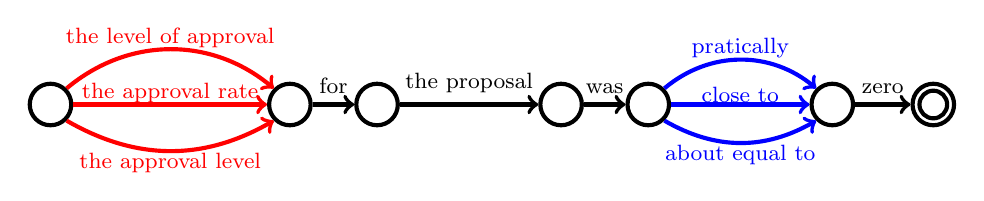
\begin{tikzpicture}	
	\tikzstyle{unit} = [circle,line width=1.5pt,draw,minimum size=1.5em]
		
		\node[unit] (u1)at (0,0){};
		\node[unit,anchor=west](u2) at ([xshift=7em]u1.east){};
		\node[unit,anchor=west](u3) at ([xshift=1.5em]u2.east){};
		\node[unit,anchor=west](u4) at ([xshift=5em]u3.east){};
		\node[unit,anchor=west](u5) at ([xshift=1.5em]u4.east){};
		\node[unit,anchor=west](u6) at ([xshift=5em]u5.east){};
		\node[unit,anchor=west,line width=1.5pt](u7) at ([xshift=2em]u6.east){};
		\node[unit,anchor=west,line width=1.5pt,minimum size=1em](u8) at ([xshift=2.25em]u6.east){};
		
		\draw[->,out=40,in=140,red,line width=1.5pt] (u1.north east) to  node[inner sep=0pt,color=red,above]{\footnotesize the level of approval}(u2.north west);
		\draw[->,red,line width=1.5pt](u1.east)-- node[inner sep=0pt,color=red,above]{\footnotesize the approval rate}(u2.west);
		\draw[->,out=-30,in=-150,red,line width=1.5pt] (u1.south east) to  node[inner sep=0pt,color=red,below]{\footnotesize the approval level}(u2.south west);
		\draw[->,line width=1.5pt](u2.east) -- node[above]{\footnotesize for} (u3.west);
		\draw[->,line width=1.5pt](u3.east) -- node[above]{\footnotesize the proposal} (u4.west);
		\draw[->,line width=1.5pt](u4.east) -- node[above]{\footnotesize was} (u5.west);
		\draw[->,out=40,in=140,blue,line width=1.5pt] (u5.north east) to  node[inner sep=0pt,color=blue,above]{\footnotesize pratically}(u6.north west);
		\draw[->,blue,line width=1.5pt](u5.east)-- node[inner sep=0pt,color=blue,above]{\footnotesize close to}(u6.west);
		\draw[->,out=-30,in=-150,blue,line width=1.5pt] (u5.south east) to  node[inner sep=0pt,color=blue,below]{\footnotesize about equal to}(u6.south west);
		\draw[->,line width=1.5pt](u6.east) -- node[above]{\footnotesize zero} (u7.west);
\end{tikzpicture}

   \caption{HyTER中参考答案集的表示方式}
   \label{fig:4-7}
\end{figure}
%----------------------------------------------

\parinterval 从图\ref{fig:4-7}中可以看出,HyTER方法通过构造同义单元的方式,可以列举出译文中每个片段的所有可能的表示方式,从而增大参考答案的数量,图\ref{fig:4-7}中的每一条路径都代表一个参考答案。但是这种对参考答案集的编码方式存在问题,同义单元之间的组合往往存在一定的限制关系\upcite{DBLP:conf/tsd/BojarMTZ13},使用HyTER方法会导致参考答案集中包含有错误的参考答案。

\begin{example}
将中文“市政府批准了一项新规定”分别翻译为英语和捷克语,使用HyTER构造的参考答案集分别如图\ref{fig:4-8}(a)和(b)所示\upcite{DBLP:conf/tsd/BojarMTZ13}:
\label{eg:4-6}
\end{example}

%----------------------------------------------
\begin{figure}[htp]
    \centering
\subfigure[\small{英语参考答案集表示}]{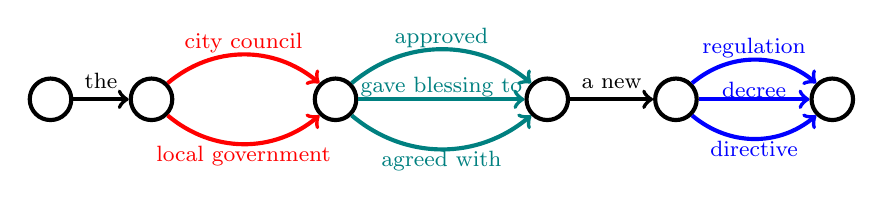
\begin{tikzpicture}	
	\tikzstyle{unit} = [circle,line width=1.5pt,draw,minimum size=1.5em]
		
		\node[unit] (u1)at (0,0){};
		\node[unit,anchor=west](u2) at ([xshift=2em]u1.east){};
		\node[unit,anchor=west](u3) at ([xshift=5em]u2.east){};
		\node[unit,anchor=west](u4) at ([xshift=6em]u3.east){};
		\node[unit,anchor=west](u5) at ([xshift=3em]u4.east){};
		\node[unit,anchor=west](u6) at ([xshift=4em]u5.east){};
		
		\draw[->,line width=1.5pt](u1.east) -- node[above]{\footnotesize the} (u2.west);
		\draw[->,out=40,in=140,red,line width=1.5pt] (u2.north east) to  node[inner sep=0pt,color=red,above]{\footnotesize city council}(u3.north west);
		\draw[->,out=-40,in=-140,red,line width=1.5pt] (u2.south east) to  node[inner sep=0pt,color=red,below]{\footnotesize local government}(u3.south west);
		
		\draw[->,out=40,in=140,teal,line width=1.5pt] (u3.north east) to  node[inner sep=0pt,color=teal,above]{\footnotesize approved}(u4.north west);
		\draw[->,teal,line width=1.5pt](u3.east)-- node[inner sep=0pt,color=teal,above]{\footnotesize gave blessing to}(u4.west);
		\draw[->,out=-40,in=-140,teal,line width=1.5pt] (u3.south east) to  node[inner sep=0pt,color=teal,below]{\footnotesize agreed with}(u4.south west);
		\draw[->,line width=1.5pt](u4.east) -- node[above]{\footnotesize a new} (u5.west);
		
		\draw[->,out=40,in=140,blue,line width=1.5pt] (u5.north east) to  node[inner sep=0pt,color=blue,above]{\footnotesize regulation}(u6.north west);
		\draw[->,blue,line width=1.5pt](u5.east)-- node[inner sep=0pt,color=blue,above]{\footnotesize decree}(u6.west);
		\draw[->,out=-40,in=-140,blue,line width=1.5pt] (u5.south east) to  node[inner sep=0pt,color=blue,below]{\footnotesize directive}(u6.south west);
		
\end{tikzpicture}
}
\subfigure[\small{捷克语参考答案集表示}]{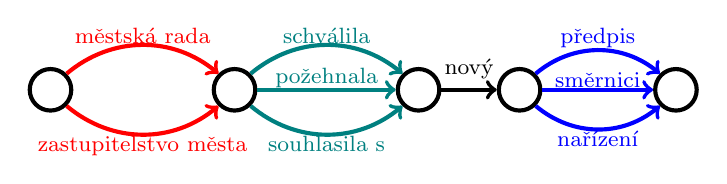
\begin{tikzpicture}	
	\tikzstyle{unit} = [circle,line width=1.5pt,draw,minimum size=1.5em]
		
		\node[unit] (u1)at (0,0){};
		\node[unit,anchor=west](u2) at ([xshift=5em]u1.east){};
		\node[unit,anchor=west](u3) at ([xshift=5em]u2.east){};
		\node[unit,anchor=west](u4) at ([xshift=2em]u3.east){};
		\node[unit,anchor=west](u5) at ([xshift=4em]u4.east){};
		
		\draw[->,out=40,in=140,red,line width=1.5pt] (u1.north east) to  node[inner sep=0pt,color=red,above]{\footnotesize městská rada}(u2.north west);
		\draw[->,out=-40,in=-140,red,line width=1.5pt] (u1.south east) to  node[inner sep=0pt,color=red,below]{\footnotesize zastupitelstvo města}(u2.south west);
		
		\draw[->,out=40,in=140,teal,line width=1.5pt] (u2.north east) to  node[inner sep=0pt,color=teal,above]{\footnotesize schválila}(u3.north west);
		\draw[->,teal,line width=1.5pt](u2.east)-- node[inner sep=0pt,color=teal,above]{\footnotesize požehnala}(u3.west);
		\draw[->,out=-40,in=-140,teal,line width=1.5pt] (u2.south east) to  node[inner sep=0pt,color=teal,below]{\footnotesize souhlasila s}(u3.south west);
		\draw[->,line width=1.5pt](u3.east) -- node[above]{\footnotesize nový} (u4.west);
		
		\draw[->,out=40,in=140,blue,line width=1.5pt] (u4.north east) to  node[inner sep=0pt,color=blue,above]{\footnotesize předpis}(u5.north west);
		\draw[->,blue,line width=1.5pt](u4.east)-- node[inner sep=0pt,color=blue,above]{\footnotesize směrnici}(u5.west);
		\draw[->,out=-40,in=-140,blue,line width=1.5pt] (u4.south east) to  node[inner sep=0pt,color=blue,below]{\footnotesize nařízení}(u5.south west);
		
\end{tikzpicture}
}
   \caption{使用HyTER构造的参考答案集}
   \label{fig:4-8}
\end{figure}
%----------------------------------------------

\parinterval 但是在捷克语中主语“městská rada”或是“zastupitelstvo města”的性别必须由动词来反映,那么上述捷克语的参考答案集中有部分存在语法错误。为了避免此类现象的出现,研究人员在同义单元中加入了将同义单元组合在一起必须满足的限制条件\upcite{DBLP:conf/tsd/BojarMTZ13},从而在增大参考答案集的同时确保了每个参考答案的准确性

\parinterval 将参考答案集扩大后,可以继续沿用BLEU或NIST等基于$n$元语法的方法进行自动评价,但是传统方法往往会忽略多重参考答案中的重复信息,于是对每个$n$元语法进行加权的自动评价方法被提出\upcite{DBLP:conf/eamt/QinS15}。该方法根据每个$n$元语法单元的长度、在参考答案集中出现的次数、被虚词(如“the”,“by”,“a”等)分开后的分散度等方面,确定其在计算最终分数时所占的权重。以BLEU方法为例(\ref{sec:ngram-eval}节),可以将式\eqref{eq:4-7}改写为:
\begin{eqnarray}
\textrm{BLEU} &=& \textrm {BP} \cdot {\textrm{exp}}(\sum\limits_{n = 1}^N {{w_n} \cdot \log ({I}_n \cdot \funp{P}_n} ))
\label{eq:4-14}\\
{I}_n &=& n\textrm{-gram}_{\textrm {diver}} \cdot \log (n + \frac{M}{\textrm{count}_{\textrm{ref}}})
\label{eq:4-15}
\end{eqnarray}

\noindent 其中,${I}_n$即为为某个$n$元语法单元分配的权重,$M$为参考答案集中出现该$n$-gram中的参考答案数量,$\textrm{count}_{\textrm{ref}}$ 为参考答案集大小。$n\textrm{-gram}_{\textrm{diver}}$为该$n$-gram的分散度,用$n$-gram种类数量与语法单元总数的比值计算。

\parinterval 需要注意的是,HyTER方法对参考译文的标注有特殊要求,因此需要单独培训译员并开发相应的标注系统。这在一定程度上也增加了该方法被使用的难度。

%----------------------------------------------------------------------------------------
%    NEW SUBSUB-SECTION
%----------------------------------------------------------------------------------------

\subsubsection{2.利用分布式表示进行质量评价}

\parinterval {\small\bfnew{词嵌入}}\index{词嵌入}(Word Embedding\index{Word Embedding})技术是近些年自然语言处理中的重要成果,其思想是把每个单词映射为多维实数空间中的一个点(具体表现为一个实数向量),这种技术也被称作单词的{\small\bfnew{分布式表示}}\index{分布式表示}(Distributed Representation\index{Distributed Representation})。在这项技术中,单词之间的关系可以通过空间的几何性质进行刻画,意义相近的单词之间的欧式距离也十分相近(单词分布式表示的具体内容,将在书的{\chapternine} 详细介绍,在此不再赘述)。

\parinterval 受词嵌入技术的启发,研究人员尝试借助参考答案和机器译文的分布式表示来进行译文质量评价,为译文质量评价提供了新思路。在自然语言的上下文中,表示是与每个单词、句子或文档相关联的数学对象。这个对象通常是一个向量,其中每个元素的值在某种程度上描述了相关单词、句子或文档的语义或句法属性。基于这个想法,研究人员提出了{\small\sffamily\bfseries{分布式表示评价度量}}\index{分布式表示评价度量}(Distributed Representations Evaluation Metrics,DREEM)\index{DREEM}\upcite{DBLP:conf/acl/ChenG15}。这种方法将单词或句子的分布式表示映射到连续的低维空间,发现在该空间中,具有相似句法和语义属性的单词彼此接近,类似的结论也出现在相关工作中,如参考文献\cite{bengio2003a,DBLP:conf/emnlp/SocherPHNM11,DBLP:conf/emnlp/SocherPWCMNP13}所示。而这个特点可以被应用到译文质量评估中。

\parinterval 在DREEM中,分布式表示的选取是一个十分关键的问题,理想的情况下,分布式表示应该涵盖句子在词汇、句法、语法、语义、依存关系等各个方面的信息。目前常见的分布式表示方式如表\ref{tab:4-2}所示。除此之外,还可以通过词袋模型、循环神经网络等将词向量表示转换为句子向量表示。

\parinterval DREEM方法中选取了能够反映句子中使用的特定词汇的One-hot向量、能够反映词汇信息的词嵌入向量\upcite{bengio2003a}、能够反映句子的合成语义信息的{\small\sffamily\bfseries{递归自动编码}}\index{递归自动编码}(Recursive Auto-encoder Embedding,RAE)\index{Recursive Auto-encoder Embedding},这三种表示级联在一起,最终形成句子的向量表示。在得到机器译文和参考答案的上述分布式表示后,利用余弦相似度和长度惩罚对机器译文质量进行评价。机器译文$o$和参考答案$g$之间的相似度如公式\eqref{eq:4-16}所示,其中${v_i}(o)$和${v_i}(g)$分别是机器译文和参考答案的向量表示中的第$i$ 个元素,$N$是向量表示的维度大小。
\begin{eqnarray}
\textrm {cos}(t,r) &=& \frac{{\sum\limits_{i = 1}^N {{v_i}(o) \cdot {v_i}(g)} }}{{\sqrt {\sum\limits_{i = 1}^N {v_i^2(o)} } \sqrt {\sum\limits_{i = 1}^N {v_i^2(g)} } }}
\label{eq:4-16}
\end{eqnarray}
\begin{table}[htp]{
\begin{center}
\caption{常见的单词及句子分布表示}
{
\begin{tabular}{l|l}
单词分布表示 & 句子分布表示 \\
\hline
\rule{0pt}{10pt} One-hot词向量 & RAE编码\upcite{DBLP:conf/emnlp/SocherPHNM11} \\
\rule{0pt}{10pt} Word2Vec词向量\upcite{DBLP:journals/corr/abs-1301-3781} & Doc2Vec向量\upcite{DBLP:conf/icml/LeM14}  \\
\rule{0pt}{10pt} Prob-fasttext词向量\upcite{DBLP:conf/acl/AthiwaratkunW17} & ELMO预训练句子表示\upcite{Peters2018DeepCW} \\
\rule{0pt}{10pt} GloVe词向量\upcite{DBLP:conf/emnlp/PenningtonSM14} & GPT句子表示\upcite{radford2018improving} \\
\rule{0pt}{10pt} ELMO预训练词向量\upcite{Peters2018DeepCW} & BERT预训练句子表示\upcite{devlin2019bert} \\
\rule{0pt}{10pt} BERT预训练词向量\upcite{devlin2019bert} & Skip-thought向量\upcite{DBLP:conf/nips/KirosZSZUTF15} \\
\end{tabular}
\label{tab:4-2}
}
\end{center}
}\end{table}

\parinterval 在此基础上,DREEM方法还引入了长度惩罚项,对与参考答案长度相差太多的机器译文进行惩罚,长度惩罚项如公式\eqref{eq:4-17}所示,其中${l_o}$和${l_g}$分别是机器译文和参考答案长度:
\begin{eqnarray}
\textrm{BP} &=& \left\{ \begin{array}{l}
\exp (1 - {{{l_g}} \mathord{\left/
 {\vphantom {{{l_g}} {{l_o}}}} \right.
 \kern-\nulldelimiterspace} {{l_o}}})\quad {l_o} < {l_g}\\
\exp (1 - {{{l_o}} \mathord{\left/
 {\vphantom {{{l_o}} {{l_g}}}} \right.
 \kern-\nulldelimiterspace} {{l_g}}})\quad {l_o} \ge {l_g}
\end{array} \right.
\label{eq:4-17}
\end{eqnarray}

\parinterval 机器译文的最终得分如下,其中$\alpha$是一个需要手动设置的参数:
\begin{eqnarray}
\textrm{score}(o,g) &=& \textrm{cos}{^\alpha }(o,g) \times \textrm{BP}
\label{eq:4-18}
\end{eqnarray}

\parinterval 本质上,分布式表示是一种对句子语义的一种统计表示。因此,它可以帮助评价系统捕捉一些从简单的词或者句子片段中不易发现的现象,进而进行更深层的句子匹配。

\parinterval 在DREEM方法取得成功后,基于词嵌入的词对齐自动评价方法被提出\upcite{DBLP:journals/corr/MatsuoKS17},该方法中先得到机器译文与参考答案的词对齐关系后,通过对齐关系中两者的词嵌入相似度来计算机器译文与参考答案的相似度,公式如\eqref{eq:4-19}。其中,$o$是机器译文,$g$是参考答案,$m$表示译文$o$的长度,$l$表示参考答案$g$的长度,函数$\varphi(o,g,i,j)$用来计算$o$中第$i$个词和$g$中第$j$个词之间对齐关系的相似度。:
\begin{eqnarray}
\textrm{ASS}(o,g) &=& \frac{1}{{m \cdot l}}\sum\limits_{i = 1}^{m} {\sum\limits_{j = 1}^{l} {\varphi (o,g,i,j)} }
\label{eq:4-19}
\end{eqnarray}

\parinterval 此外,将分布式表示与相对排序融合也是一个很有趣的想法\upcite{DBLP:journals/csl/GuzmanJMN17},在这个尝试中,研究人员利用分布式表示提取参考答案和多个机器译文中的句法信息和语义信息,利用神经网络模型对多个机器译文进行排序。

\parinterval 在基于分布式表示的这类译文质量评价方法中,译文和参考答案的所有词汇信息和句法语义信息都被包含在句子的分布式表示中,克服了单一参考答案的限制。但是同时也带来了新的问题,一方面将句子转化成分布式表示使评价过程变得不那么具有可解释性,另一方面分布式表示的质量也会对评价结果有较大的影响。

%----------------------------------------------------------------------------------------
%    NEW SUB-SECTION
%----------------------------------------------------------------------------------------

\subsection{相关性与显著性}

\parinterval 近年来,随着多种有参考答案的自动评价方法的提出,译文质量评价已经渐渐从大量的人力工作中解脱转而依赖于自动评价技术。然而,一些自动评价结果的可靠性、置信性以及参考价值仍有待商榷。自动评价结果与人工评价结果的相关性以及其自身的统计显著性,都是衡量其可靠性、置信性以及参考价值的重要标准。

%----------------------------------------------------------------------------------------
%    NEW SUBSUB-SECTION
%----------------------------------------------------------------------------------------

\subsubsection{1. 自动评价与人工评价的相关性}

\parinterval {\small\sffamily\bfseries{相关性}}\index{相关性}(Correlation)\index{Correlation}是统计学中的概念,当两个变量之间存在密切的依赖或制约关系,但却无法确切地表示时,可以认为两个变量之间存在“相关关系”,并往往用“相关性”作为衡量关系密切程度的标准\upcite{pearson1920notes}。对于相关关系,虽然无法求解两个变量之间确定的函数关系,但是通过大量的观测数据,能够发现变量之间存在的统计规律性,而“相关性”也同样可以利用统计手段获取。

\parinterval 在机器译文质量评价工作中,相比人工评价,有参考答案的自动评价具有效率高、成本低的优点,因而广受机器翻译系统研发人员青睐。在这种情况下,自动评价结果的可信度一般取决于它们与可靠的人工评价之间的相关性。随着越来越多有参考答案的自动评价方法的提出,“与人工评价之间的相关性”也被视为衡量一种新的自动评价方法是否可靠的衡量标准。

\parinterval 很多研究工作中都曾对BLEU、NIST等有参考答案的自动评价与人工评价的相关性进行研究和讨论,其中也有很多工作对“相关性”的统计过程作过比较详细的阐述。在“相关性”的统计过程中,一般是分别利用人工评价方法和某种有参考答案的自动评价方法对若干个机器翻译系统的输出进行等级评价\upcite{coughlin2003correlating}或是相对排序\upcite{popescu2003experiment},从而对比两种评价手段的评价结果是否一致。该过程中的几个关键问题可能会对最终结果产生影响。

\begin{itemize}
\vspace{0.5em}
\item {\small\sffamily\bfseries{源语言句子的选择}}。由于机器翻译系统一般以单句作为翻译单元,因而评价过程中涉及的源语言句子是脱离上下文语境的单句\upcite{coughlin2003correlating}。
\vspace{0.5em}
\item {\small\sffamily\bfseries{人工评估结果的产生}}。人工评价过程中采用只提供标准高质量参考答案的单语评价方法,由多位评委对译文质量做出评价后进行平均作为最终的人工评价结果\upcite{coughlin2003correlating}。
\vspace{0.5em}
\item {\small\sffamily\bfseries{自动评价中参考答案的数量}}。在有参考答案的自动评价过程中,为了使评价结果更加准确,一般会设置多个参考答案。参考答案数量的设置会对自动评价与人工评价的相关性产生影响,也有很多工作对此进行了研究。例如人们发现有参考答案的自动评价方法在区分人类翻译和机器翻译时,设置4个参考答案的区分效果远远高于2个参考答案\upcite{culy2003limits};也有人曾专注于研究怎样设置参考答案数量能够产生最高的相关性\upcite{finch2004using}。
\vspace{0.5em}
\item {\small\sffamily\bfseries{自动评价中参考答案的质量}}。从直觉上,自动评价中参考答案的质量一般会影响最终的评价结果,从而对相关性的计算产生影响。然而,有相关实验表明,只要参考答案的质量不是过分低劣,很多情况下自动评价都能得到相同的评价结果\upcite{DBLP:conf/coling/HamonM08}。
\vspace{0.5em}
\end{itemize}

\parinterval 目前在机器译文质量评价的领域中,有很多研究工作尝试比较各种有参考答案的自动评价方法(主要以BLEU、NIST等基于$n$-gram的方法为主)与人工评价方法的相关性。整体来看,这些方法与人工评价具有一定的相关性,自动评价结果能够较好地反映译文质量\upcite{coughlin2003correlating,doddington2002automatic}。

\parinterval 但是也有相关研究指出,不应该对有参考答案的自动评价方法过于乐观,而应该存谨慎态度,因为目前的自动评价方法对于流利度的评价并不可靠,同时参考答案的体裁和风格往往会对自动评价结果产生很大影响\upcite{culy2003limits}。同时,有研究人员提出,机器翻译研究过程中,在忽略实际示例翻译的前提下,BLEU分数的提高并不意味着翻译质量的真正提高,而在一些情况下,为了实现翻译质量的显著提高,并不需要提高BLEU分数\upcite{callison2006re}。

%----------------------------------------------------------------------------------------
%    NEW SUBSUB-SECTION
%----------------------------------------------------------------------------------------

\subsubsection{2. 自动评价方法的统计显著性}


\parinterval 使用自动评价的目的是比较不同系统之间性能的差别。比如,对某个机器翻译系统进行改进后,它的BLEU值从40.0$\%$提升到40.5$\%$,能否说改进后的系统真的比改进前的翻译品质更好吗?实际上,这也是统计学中经典的{\small\sffamily\bfseries{统计假设检验}}\index{统计假设检验}(Statistical Hypothesis Testing)\index{Statistical Hypothesis Testing}问题\upcite{akaike1974new}。统计假设检验的基本原理是:如果对样本总体的某种假设是真的,那么不支持该假设的小概率事件几乎是不可能发生的;一旦这种小概率事件在某次试验中发生了,那就有理由拒绝原始的假设。例如,对于上面提到了例子,可以假设:

\begin{itemize}
\vspace{0.5em}
\item {\small\sffamily\bfseries{原始假设}}:改进后比改进前翻译品质更好;
\vspace{0.5em}
\item {\small\sffamily\bfseries{小概率事件}}(备择假设):改进后和改进前比,翻译品质相同甚至更差。
\vspace{0.5em}
\end{itemize}

\parinterval 统计假设检验的流程如图\ref{fig:4-13}所示。其中的一个关键步骤是检验一个样本集合中是否发生了小概率事件。但是,怎样才算是小概率事件呢?比如,可以定义概率不超过0.1的事件就是小概率事件,甚至可以定义这个概率为0.05、0.01。通常,这个概率被记为$\alpha$,也就是常说的{\small\sffamily\bfseries{显著性水平}}\index{显著性水平}(Significance Level)\index{Significance Level}。 而显著性水平更准确的定义是“去真错误”的概率,即:原假设为真但是拒绝了它的概率。

%----------------------------------------------
\begin{figure}[htp]
    \centering
	\usetikzlibrary{shapes.geometric}

\begin{tikzpicture}
	\node[font=\footnotesize] (overall) at (0,0){\small\bfnew{总 \ \ \ \ 体}};
	\node[anchor=north,font=\footnotesize] (hypo) at ([yshift=-3em]overall.south){某种假设};
	\coordinate (A) at ([yshift=-3.5em,xshift=-1.6em]overall);
	\coordinate (B) at ([yshift=0.3em,xshift=0.3em]A);
	\draw[] (B)  .. controls +(east:1.3em) and +(west:0.3em) .. ([xshift=1.5em,yshift=2em]B) .. controls +(east:0.3em) and +(west:1.3em) .. ([xshift=3em]B);
	\draw[<->] ([yshift=2.4em]A) -- (A) -- ([xshift=3.7em]A);
	\begin{pgfonlayer}{background}
        	\node [draw,thick,rectangle,inner sep=0.5em,rounded corners=2pt,fill=red!30,drop shadow] [fit = (overall)(hypo)] (box1) {};
    \end{pgfonlayer}
	\node[draw,fill=yellow!30,thick,anchor=west,font=\footnotesize,align=center,drop shadow](sample) at ([xshift=4em]box1.east){样本\\观察结果};
	\node[anchor=west,draw,diamond,fill=green!30!white,drop shadow,aspect=2,font=\scriptsize,align=center,inner sep=1pt,thick] (judge) at ([xshift=3em]sample.east){小概率事件\\发生?};
	\node[draw,fill=blue!30,thick,drop shadow,anchor=west,font=\footnotesize,align=center,thick](refuse) at ([xshift=6em]judge.north){拒绝原假设};
	\node[draw,fill=blue!30,thick,drop shadow,anchor=west,font=\footnotesize,align=center,thick](accept) at ([xshift=6em]judge.south){接受原假设};
	\draw[->,thick] (box1.east) -- node[above,font=\scriptsize]{抽样}(sample.west);
	\draw[->,thick] (sample.east) -- node[above,font=\scriptsize]{检验}(judge.west);
	\draw[->,thick] (judge.north) -- node[above,font=\scriptsize]{是}(refuse.west);
	\draw[->,thick] (judge.south) -- node[below,font=\scriptsize]{否}(accept.west);
\end{tikzpicture}

   \caption{统计假设检验的流程}
   \label{fig:4-13}
\end{figure}
%----------------------------------------------

\parinterval 回到机器翻译的问题中来。一个更加基础的问题是:一个系统评价结果的变化在多大范围内是不显著的。利用假设检验的原理,这个问题可以被描述为:评价结果落在$[x-d,x+d]$区间的置信度是$1-\alpha$。换句话说,当系统性能落在$[x-d, x+d]$外,就可以说这个结果与原始的结果有显著性差异。这里$x$通常是系统译文的BLEU计算结果,$[x-d,x+d]$是其对应的置信区间。而$d$和$\alpha$有很多计算方法,比如,如果假设评价结果服从正态分布,可以简单的计算$d$。
\begin{eqnarray}
d&=&t \frac{s}{\sqrt{n}}
\label{eq:4-21}
\end{eqnarray}

\noindent 其中,$s$是标准差,$n$是样本数。$t$是一个统计量,它与假设检验的方式、显著性水平、样本数量有关。

\parinterval 而机器翻译评价使用假设检验的另一个问题是如何进行抽样。需要注意的是,这里的样本是指一个机器翻译的测试集,因为BLEU等指标都是在整个测试集上计算的,而非简单的通过句子级评价结果进行累加。为了保证假设检验的充分性,需要构建多个测试集,以模拟从所有潜在的测试集空间中采样的行为。

\parinterval 最常用的方法是使用Bootstrap重采样技术\upcite{DBLP:books/sp/EfronT93}从一个固定测试集中采样不同的句子组成不同的测试集,之后在这些测试集上进行假设检验\upcite{DBLP:conf/emnlp/Koehn04}。此后,有工作指出了Bootstrap重采样方法存在隐含假设的不合理之处,并提出了使用近似随机化\upcite{noreen1989computer}方法计算自动评价方法统计显著性\upcite{DBLP:conf/acl/RiezlerM05}。另有研究工作着眼于研究自动评价结果差距大小、测试集规模、系统相似性等因素对统计显著性的影响,以及在不同领域的测试语料中计算的统计显著性是否具有通用性的问题\upcite{DBLP:conf/emnlp/Berg-KirkpatrickBK12}。

\parinterval 在所有自然语言处理系统的结果对比中,显著性检验是十分必要的。很多时候不同系统性能的差异性很小,因此需要确定一些微小的进步是否是“真”的,还是只是一些随机事件。但是从实践的角度看,当某个系统性能的提升达到一个绝对值,这种性能提升效果往往是显著的。比如,在机器翻译,BLEU提升0.5$\%$一般都是比较明显的进步。也有研究对这种观点进行了论证,也发现其中具有一定的科学性\upcite{DBLP:conf/emnlp/Berg-KirkpatrickBK12}。因此,在机器翻译系统研发中类似的方式也是可以采用的。

%----------------------------------------------------------------------------------------
%    NEW SECTION
%----------------------------------------------------------------------------------------

\sectionnewpage
\section{无参考答案的自动评价}

\parinterval 无参考答案自动评价在机器翻译领域又被称作{\small\sffamily\bfseries{质量评估}}\index{质量评估}(Quality Estimation,\\QE)\index{Quality Estimation}。与传统的译文质量评价方法不同,质量评估旨在不参照标准译文的情况下,对机器翻译系统的输出在单词、短语、句子、文档等各个层次进行评价。

\parinterval 人们对于无参考答案自动评价的需求大多来源于机器翻译的实际应用。例如,在机器翻译的译后编辑过程中,译员不仅仅希望了解机器翻译系统的整体翻译质量,还需要了解该系统在某个句子上的表现如何:该机器译文的质量是否很差?需要修改的内容有多少?是否值得进行后编辑?这时,译员更加关注系统在单个数据点上(比如一段话)的可信度而非系统在测试数据集上的平均质量。这时,太多的人工介入就无法保证使用机器翻译所带来的高效性,因此在机器翻译输出译文的同时,需要质量评估系统给出对译文质量的预估结果。这些需求也促使研究人员在质量评估问题上投入了更多的研究力量。包括WMT、CCMT等知名机器翻译评测中也都设置了相关任务,受到了业界的关注。

%----------------------------------------------------------------------------------------
%    NEW SUB-SECTION
%----------------------------------------------------------------------------------------

\subsection{质量评估任务}

\parinterval 质量评估任务本质上是通过预测一个能够反映评价单元的质量标签,在各个层次上对译文进行质量评价。在上文中已经提到,质量评估任务通常被划分为单词级、短语级、句子级和文档级,在接下来的内容中,将对各个级别的任务进行更加详细的介绍。

%----------------------------------------------------------------------------------------
%    NEW SUBSUB-SECTION
%----------------------------------------------------------------------------------------

\subsubsection{1.单词级质量评估}

\parinterval 机器翻译系统在翻译某个句子时,会出现各种类型的错误,这些错误多是一些单词翻译问题,例如单词出现歧义、单词漏译、单词错译、词形转化错误等等。单词级质量评价以单词为评估单元,目的是确定译文句子中每个单词的所在位置是否存在翻译错误和单词漏译现象。

\parinterval 单词级质量评估任务可以被定义为:参照源语言句子,以单词为评价单位,自动标记出机器译文中的错误。其中的“错误”包括单词错译、单词词形错误、单词漏译等。在单词级质量评估任务中,输入是机器译文和源语言句子,输出是一系列标签序列,即图\ref{fig:4-11}中的Source tags、MT tags、Gap tags,标签序列中的每个标签对应翻译中的每个单词(或其间隙),并表明该位置是否出现错误。

%----------------------------------------------
\begin{figure}[htp]
    \centering
	\definecolor{ugreen}{rgb}{0,0.5,0}

\begin{tikzpicture}[scale=0.6]
	\tikzstyle{unit} = [draw,inner sep=3pt,font=\footnotesize,minimum height=1.2em,drop shadow={shadow xshift=0.1em,shadow yshift=-0.15em}]
	\tikzstyle{bad_tag} = [fill=red!15,inner sep=1pt,align=center,font=\scriptsize,text=red!80]
	\tikzstyle{ok_tag} = [fill=ugreen!15,inner sep=1pt,align=center,font=\scriptsize,text=ugreen!80]
	
	\coordinate (o) at (0, 0);
	
	\node[anchor=west,inner sep=0pt,align=center,font=\scriptsize] (n1_1) at ([yshift=5.5em]o.east){\textbf{Source}};
	\node[unit,anchor=west,fill=green!30](n1_2) at ([xshift=8.4em]n1_1.east){Draw};
	\node[unit,anchor=west,fill=green!30](n1_3) at ([xshift=0.8em]n1_2.east){or};
	\node[unit,anchor=west,fill=green!30](n1_4) at ([xshift=0.8em]n1_3.east){select};
	\node[unit,anchor=west,fill=green!30](n1_5) at ([xshift=0.8em]n1_4.east){a};
	\node[unit,anchor=west,fill=green!30](n1_6) at ([xshift=0.8em]n1_5.east){line};
	\node[unit,anchor=west,fill=green!30](n1_7) at ([xshift=0.8em]n1_6.east){.};
	
	\node[anchor=west,inner sep=0pt,align=center,font=\scriptsize] (n2_1) at (o.east){\textbf{PE}};
	\node[unit,anchor=west,fill=red!30](n2_2) at ([xshift=1.8em]n2_1.east){Zeichnen};
	\node[unit,anchor=west,fill=red!30](n2_3) at ([xshift=0.8em]n2_2.east){oder};
	\node[unit,anchor=west,fill=red!30](n2_4) at ([xshift=0.8em]n2_3.east){Sie};
	\node[unit,anchor=west,fill=red!30](n2_5) at ([xshift=0.8em]n2_4.east){eine};
	\node[unit,anchor=west,fill=red!30](n2_6) at ([xshift=0.8em]n2_5.east){linie};
	\node[unit,anchor=west,fill=red!30](n2_7) at ([xshift=0.8em]n2_6.east){,};
	\node[unit,anchor=west,fill=red!30](n2_8) at ([xshift=0.8em]n2_7.east){order};
	\node[unit,anchor=west,fill=red!30](n2_9) at ([xshift=0.8em]n2_8.east){wählen};
	\node[unit,anchor=west,fill=red!30](n2_10) at ([xshift=0.8em]n2_9.east){Sie};
	\node[unit,anchor=west,fill=red!30](n2_11) at ([xshift=0.8em]n2_10.east){eine};
	\node[unit,anchor=west,fill=red!30](n2_12) at ([xshift=0.8em]n2_11.east){aus};
	\node[unit,anchor=west,fill=red!30](n2_13) at ([xshift=0.8em]n2_12.east){.};
	
	\node[anchor=west,inner sep=0pt,align=center,font=\scriptsize] (n3_1) at ([yshift=-5.5em]o.east){\textbf{MT}};
	\node[unit,anchor=west,fill=blue!30](n3_2) at ([xshift=5.5em]n3_1.east){Zeichnen};
	\node[unit,anchor=west,fill=blue!30](n3_3) at ([xshift=0.8em]n3_2.east){oder};
	\node[unit,anchor=west,fill=blue!30](n3_4) at ([xshift=0.8em]n3_3.east){wählen};
	\node[unit,anchor=west,fill=blue!30](n3_5) at ([xshift=0.8em]n3_4.east){Sie};
	\node[unit,anchor=west,fill=blue!30](n3_6) at ([xshift=0.8em]n3_5.east){eine};
	\node[unit,anchor=west,fill=blue!30](n3_7) at ([xshift=0.8em]n3_6.east){Linie};
	\node[unit,anchor=west,fill=blue!30](n3_8) at ([xshift=0.8em]n3_7.east){aus};
	\node[unit,anchor=west,fill=blue!30](n3_9) at ([xshift=0.8em]n3_8.east){.};
	
	\node[bad_tag,anchor=south] at ([yshift=2pt]n1_2.north){BAD};
	\node[bad_tag,anchor=south] at ([yshift=2pt]n1_3.north){BAD};
	\node[ok_tag,anchor=south] at ([yshift=2pt]n1_4.north){OK};
	\node[bad_tag,anchor=south] at ([yshift=2pt]n1_5.north){BAD};
	\node[bad_tag,anchor=south] at ([yshift=2pt]n1_6.north){BAD};
	\node[ok_tag,anchor=south] (tag1) at ([yshift=2pt]n1_7.north){OK};
	
	
	\node[ok_tag,anchor=north] at ([yshift=-3pt]n3_2.south){OK};
	\node[ok_tag,anchor=north] at ([yshift=-3pt]n3_3.south){OK};
	\node[ok_tag,anchor=north] at ([yshift=-3pt]n3_4.south){OK};
	\node[ok_tag,anchor=north] at ([yshift=-3pt]n3_5.south){OK};
	\node[ok_tag,anchor=north] at ([yshift=-3pt]n3_6.south){OK};
	\node[bad_tag,anchor=north] at ([yshift=-3pt]n3_7.south){BAD};
	\node[ok_tag,anchor=north] at ([yshift=-3pt]n3_8.south){OK};
	\node[ok_tag,anchor=north] (tag2) at ([yshift=-3pt]n3_9.south){OK};
		
	\node[ok_tag,anchor=north] (gap_1)at ([xshift=-3.2em,yshift=-2em]n3_2.south){OK};
	\node[bad_tag,anchor=north] (gap_2)at ([xshift=3.5em,yshift=-2em]n3_2.south){BAD};
	\node[ok_tag,anchor=north] (gap_3)at ([xshift=2.1em,yshift=-2em]n3_3.south){OK};
	\node[ok_tag,anchor=north] (gap_4)at ([xshift=3em,yshift=-2em]n3_4.south){OK};
	\node[ok_tag,anchor=north] (gap_5)at ([xshift=1.85em,yshift=-2em]n3_5.south){OK};
	\node[ok_tag,anchor=north] (gap_6)at ([xshift=2em,yshift=-2em]n3_6.south){OK};
	\node[ok_tag,anchor=north] (gap_7)at ([xshift=2.25em,yshift=-2em]n3_7.south){OK};
	\node[ok_tag,anchor=north] (gap_8)at ([xshift=1.75em,yshift=-2em]n3_8.south){OK};
	\node[ok_tag,anchor=north] (tag3) at ([xshift=1.7em,yshift=-2em]n3_9.south){OK};

	\draw[dash pattern=on 2pt off 1pt,gray,line width=1pt](gap_1.north) -- ([yshift=2em]gap_1.north);
	\draw[dash pattern=on 2pt off 1pt,gray,line width=1pt](gap_2.north) -- ([yshift=2em]gap_2.north);
	\draw[dash pattern=on 2pt off 1pt,gray,line width=1pt](gap_3.north) -- ([yshift=2em]gap_3.north);
	\draw[dash pattern=on 2pt off 1pt,gray,line width=1pt](gap_4.north) -- ([yshift=2em]gap_4.north);
	\draw[dash pattern=on 2pt off 1pt,gray,line width=1pt](gap_5.north) -- ([yshift=2em]gap_5.north);
	\draw[dash pattern=on 2pt off 1pt,gray,line width=1pt](gap_6.north) -- ([yshift=2em]gap_6.north);
	\draw[dash pattern=on 2pt off 1pt,gray,line width=1pt](gap_7.north) -- ([yshift=2em]gap_7.north);
	\draw[dash pattern=on 2pt off 1pt,gray,line width=1pt](gap_8.north) -- ([yshift=2em]gap_8.north);
	\draw[dash pattern=on 2pt off 1pt,gray,line width=1pt](tag3.north) -- ([yshift=2em]tag3.north);
	
	\draw [line width=1pt,blue!30](n1_2.south) -- (n2_2.north);
	\draw [line width=1pt,blue!30](n1_3.south) -- (n2_3.north);
	\draw [line width=1pt,blue!30](n1_4.south) -- (n2_4.north);
	\draw [line width=1pt,blue!30](n1_4.south) -- (n2_9.north);
	\draw [line width=1pt,blue!30](n1_5.south) -- (n2_5.north);
	\draw [line width=1pt,blue!30](n1_6.south) -- (n2_6.north);
	\draw [line width=1pt,blue!30](n1_7.south) -- (n2_13.north);

	\draw[line width=1pt,ugreen!60] (n2_2.south) -- (n3_2.north);
	\draw[line width=1pt,ugreen!60] (n2_3.south) -- (n3_3.north);
	\draw[line width=1pt,ugreen!60] (n2_4.south) -- (n3_5.north);
	\draw[line width=1pt,ugreen!60] (n2_5.south) -- (n3_6.north);
	\draw[line width=1pt,red!60] (n2_6.south) -- (n3_7.north);
	\draw[line width=1pt,ugreen!60] (n2_9.south) -- (n3_4.north);
	\draw[line width=1pt,ugreen!60] (n2_12.south) -- (n3_8.north);
	\draw[line width=1pt,ugreen!60] (n2_13.south) -- (n3_9.north);
	
	\node[anchor=west,inner sep=0pt,align=center,font=\scriptsize](st)  at ([xshift=14.4em]tag1.east){\textbf{Source tags}};
	\node[anchor=west,inner sep=0pt,align=center,font=\scriptsize]  at ([xshift=6.6em]tag2.east){\textbf{MT tags}};
	\node[anchor=west,inner sep=0pt,align=center,font=\scriptsize] (gt) at ([xshift=4.6em]tag3.east){\textbf{Gap tags}};
\end{tikzpicture}
   \caption{单词级质量评估任务示意图}
   \label{fig:4-11}
\end{figure}
%----------------------------------------------

\parinterval 下面以实例\ref{eg:4-7}为例介绍该任务的具体内容,在实例\ref{eg:4-7}中加入后编辑结果是方便读者理解任务内容,实际上质量评估任务在预测质量标签时并不依赖后编辑结果:

\begin{example}
单词级质量评估任务

源句(Source):Draw or select a line .(英语)

机器译文(MT):Zeichnen oder wählen Sie eine Linie aus .(德语)

后编辑结果(PE):Zeichnen oder Sie eine Linie, oder wählen Sie eine aus .(德语)

\label{eg:4-7}
\end{example}

\parinterval 单词级质量评估主要通过以下三类错误评价译文好坏:

\begin{itemize}
\vspace{0.5em}
\item {\small\sffamily\bfseries{找出译文中翻译错误的单词}}。单词级质量评估任务要求预测一个与译文等长的质量标签序列,该标签序列反映译文端的每个单词是否能够准确表达出其对应的源端单词的含义,若是可以,则标签为“OK”,反之则为“BAD”。图\ref{fig:4-11}中的连线表示单词之间的对齐关系,图\ref{fig:4-11}中的MT tags即为该过程中需要预测的质量标签序列。
\vspace{0.5em}
\item {\small\sffamily\bfseries{找出源文中导致翻译错误的单词}}。单词级质量评估任务还要求预测一个与源文等长的质量标签序列,该标签序列反映源文端的每个单词是否会导致本次翻译出现错误,若是不会,则标签为“OK”,反之则为“BAD”。图\ref{fig:4-11}中的Source tags即为该过程中的质量标签序列。在具体应用时,质量评估系统往往先预测译文端的质量标签序列,并根据源文与译文之间的对齐关系,推测源端的质量标签序列。
\vspace{0.5em}
\item {\small\sffamily\bfseries{找出在翻译句子时出现漏译现象的位置}}。单词级质量评估任务同时也要求预测一个能够捕捉到漏译现象的质量标签序列,在译文端单词的两侧位置进行预测,若某位置未出现漏译,则该位置的质量标签为“OK”,否则为“BAD”。图\ref{fig:4-11}中的Gap tags即为该过程中的质量标签序列。为了检测句子翻译中的漏译现象,需要在译文中标记缺口,即译文中的每个单词两边都各有一个“GAP”标记,如图\ref{fig:4-11}所示。
\vspace{0.5em}
\end{itemize}

%----------------------------------------------------------------------------------------
%    NEW SUBSUB-SECTION
%----------------------------------------------------------------------------------------

\subsubsection{2.短语级质量评估}

\parinterval 短语级质量评估可以看做是单词级质量评估任务的扩展:机器翻译系统引发的错误往往都是相互关联的,解码过程中某个单词出错会导致更多的错误,特别是在其局部上下文当中,以单词的“局部上下文”为基本单元进行质量评估即为短语级质量评估。

\parinterval 短语级质量评估与单词级质量评估类似,其目标是找出短语中翻译错误、短语内部语序问题及漏译问题。短语级质量评估任务可以被定义为:以若干个连续单词组成的短语为基本评估单位,参照源语言句子,自动标记出短语内部短语错误以及短语之间的是否存在漏译。其中的短语错误包括短语内部单词的错译和漏译、短语内部单词的语序错误,而漏译问题则特指短语之间的漏译错误。在短语级质量评估任务中,输入是机器译文和源语言句子,输出是一系列标签序列,即图\ref{fig:4-12}中的Phrase-target tags、Gap tags,标签序列中的每个标签对应翻译中的每个单词,并表明该位置是否出现错误。

%----------------------------------------------
\begin{figure}[htp]
    \centering
	%\usetikzlibrary{backgrounds} 
%\usetikzlibrary{fit}
\begin{tikzpicture}[scale=0.5]
	\tikzstyle{unit} = [draw,inner sep=1.2pt,font=\scriptsize,minimum height=1em]
	\tikzstyle{box} = [draw,rectangle,inner xsep=1.4pt,inner ysep=3pt]
	\tikzstyle{bad_tag} = [inner sep=1pt,align=center,font=\scriptsize,text=red,minimum height=0.8em]
	\tikzstyle{ok_tag} = [inner sep=1pt,align=center,font=\scriptsize,text=ugreen,minimum height=0.8em]
	
	\coordinate (o) at (0, 0);
	
	\node[anchor=west,inner sep=0pt,align=center,font=\scriptsize] (n1_1) at ([yshift=8em]o.east){\textbf{Source}};
	\node[unit,anchor=west,fill=green!30](n1_2) at ([xshift=2.2em]n1_1.east){Nach};
	\node[unit,anchor=west,fill=green!30](n1_3) at ([xshift=0.6em]n1_2.east){Zubereitung};
	\node[unit,anchor=west,fill=green!30](n1_4) at ([xshift=1.2em]n1_3.east){im};
	\node[unit,anchor=west,fill=green!30](n1_5) at ([xshift=0.6em]n1_4.east){Kühlschrank};
	\node[unit,anchor=west,fill=green!30](n1_6) at ([xshift=0.6em]n1_5.east){aufbewahren};
	\node[unit,anchor=west,fill=green!30](n1_7) at ([xshift=1.2em]n1_6.east){und};
	\node[unit,anchor=west,fill=green!30](n1_8) at ([xshift=0.6em]n1_7.east){innerhalb};
	\node[unit,anchor=west,fill=green!30](n1_9) at ([xshift=0.6em]n1_8.east){vonf};
	\node[unit,anchor=west,fill=green!30](n1_10) at ([xshift=0.6em]n1_9.east){24};
	\node[unit,anchor=west,fill=green!30](n1_11) at ([xshift=1.2em]n1_10.east){Stunden};
	\node[unit,anchor=west,fill=green!30](n1_12) at ([xshift=0.6em]n1_11.east){aufbrauchen};

	
	\node[anchor=west,inner sep=0pt,align=center,font=\scriptsize] (n2_1) at ([yshift=-2em]o.east){\textbf{MT}};
	\node[unit,anchor=west,fill=red!30](n2_2) at ([xshift=5em]n2_1.east){After};
	\node[unit,anchor=west,fill=red!30](n2_3) at ([xshift=0.6em]n2_2.east){reconstitution};
	\node[unit,anchor=west,fill=red!30](n2_4) at ([xshift=1.2em]n2_3.east){in};
	\node[unit,anchor=west,fill=red!30](n2_5) at ([xshift=0.6em]n2_4.east){the};
	\node[unit,anchor=west,fill=red!30](n2_6) at ([xshift=0.6em]n2_5.east){refrigerator};
	\node[unit,anchor=west,fill=red!30](n2_7) at ([xshift=1.2em]n2_6.east){and};
	\node[unit,anchor=west,fill=red!30](n2_8) at ([xshift=0.6em]n2_7.east){used};
	\node[unit,anchor=west,fill=red!30](n2_9) at ([xshift=0.6em]n2_8.east){within};
	\node[unit,anchor=west,fill=red!30](n2_10) at ([xshift=0.6em]n2_9.east){24};
	\node[unit,anchor=west,fill=red!30](n2_11) at ([xshift=1.2em]n2_10.east){hours};
	\begin{pgfonlayer}{background}
        \node [box,fill=green!5] [fit = (n1_2) (n1_3)] (box1_1) {};
        \node [box,fill=green!5] [fit = (n1_4) (n1_5) (n1_6)] (box1_2) {};
        \node [box,fill=green!5] [fit = (n1_7) (n1_8) (n1_9) (n1_10)] (box1_3) {};
        \node [box,fill=green!5] [fit = (n1_11) (n1_12) ] (box1_4) {};
        
        \node [box,fill=red!5] [fit = (n2_2) (n2_3)] (box2_1) {};
        \node [box,fill=red!5] [fit = (n2_4) (n2_5) (n2_6)] (box2_2) {};
        \node [box,fill=red!5] [fit = (n2_7) (n2_8) (n2_9) (n2_10)] (box2_3) {};
        \node [box,fill=red!5] [fit = (n2_11)] (box2_4) {};
    \end{pgfonlayer}
	
	\node[bad_tag,anchor=north] at ([yshift=-2pt]box2_1.south){BAD\_word\_order};
	\node[ok_tag,anchor=north] at ([yshift=-2pt]box2_2.south){OK};
	\node[bad_tag,anchor=north] at ([yshift=-2pt]box2_3.south){BAD};
	\node[ok_tag,anchor=north] (tag_1) at ([yshift=-2pt]box2_4.south){OK};
	
	\node[ok_tag,anchor=north] (gap_1) at ([xshift=-7em,yshift=-3em]box2_1.south){OK};
	\node[bad_tag,anchor=north] (gap_2) at ([xshift=7em,yshift=-3em]box2_1.south){BAD\_omission};
	\node[ok_tag,anchor=north] (gap_3) at ([xshift=6.8em,yshift=-3em]box2_2.south){OK};
	\node[ok_tag,anchor=north] (gap_4) at ([xshift=7.5em,yshift=-3em]box2_3.south){OK};
	\node[ok_tag,anchor=north] (tag_2) at ([xshift=2.5em,yshift=-3em]box2_4.south){OK};

	
	\node[anchor=west,inner sep=0pt,align=center,font=\scriptsize] at ([xshift=5.2em]tag_1.east){\textbf{Phrase-target tags}};
	
	\node[anchor=west,inner sep=0pt,align=center,font=\scriptsize] at ([xshift=8.4em]tag_2.east){\textbf{Gap tags}};
	
	\draw[blue!30,line width=1pt] (n1_2.south) -- (n2_2.north);
	\draw[blue!30,line width=1pt] (n1_2.south) -- (n2_3.north);
	\draw[blue!30,line width=1pt] (n1_3.south) -- (n2_3.north);
	\draw[blue!30,line width=1pt] (n1_4.south) -- (n2_4.north);
	\draw[blue!30,line width=1pt] (n1_4.south) -- (n2_5.north);
	\draw[blue!30,line width=1pt] (n1_4.south) -- (n2_6.north);
	\draw[blue!30,line width=1pt] (n1_5.south) -- (n2_6.north);
	\draw[blue!30,line width=1pt] (n1_6.south) -- (n2_6.north);
	\draw[blue!30,line width=1pt] (n1_7.south) -- (n2_7.north);
	\draw[blue!30,line width=1pt] (n1_8.south) -- (n2_9.north);
	\draw[blue!30,line width=1pt] (n1_9.south) -- (n2_9.north);
	\draw[blue!30,line width=1pt] (n1_10.south) -- (n2_10.north);
	\draw[blue!30,line width=1pt] (n1_11.south) -- (n2_11.north);
	\draw[blue!30,line width=1pt] (n1_12.south) -- (n2_11.north);	
	
	\draw[dotted,thick](gap_1.north) -- ([yshift=3em]gap_1.north);
	\draw[dotted,thick](gap_2.north) -- ([yshift=3em]gap_2.north);
	\draw[dotted,thick](gap_3.north) -- ([yshift=3em]gap_3.north);
	\draw[dotted,thick](gap_4.north) -- ([yshift=3em]gap_4.north);
	\draw[dotted,thick](tag_2.north) -- ([yshift=3em]tag_2.north);
	
	
\end{tikzpicture}

   \caption{短语级质量评估任务示意图}
   \label{fig:4-12}
\end{figure}
%----------------------------------------------

\parinterval 下面以实例\ref{eg:4-8}为例介绍该任务的具体内容:

\begin{example}
短语级质量评估任务(短语间用 || 分隔)

源句(Source):Nach Zubereitung || im Kühlschrank aufbewahren || und innerha-

\hspace{7.3em}lb von 24 || Stunden aufbrauchen .(德语)

机器译文(MT):After reconstitution || in the refrigerator || and used within 24 ||

 \hspace{8em}hours . (英语)
\label{eg:4-8}
\end{example}

\parinterval 短语级质量评估任务主要通过以下两类类错误评价译文好坏:

\begin{itemize}
\vspace{0.5em}
\item {\small\sffamily\bfseries{找出译文中翻译错误的短语}}。要求预测出一个能够捕捉短语内部单词翻译错误、单词漏译以及单词顺序错误的标签序列。该序列中每个标签都对应着一个短语,若是短语不存在任何错误,则标签为“OK”;若是短语内部存在单词翻译错误和单词漏译,则标签为“BAD”;若短语内部的单词顺序存在问题,则标签为“BAD\_word\_order”。图\ref{fig:4-12}中的连线表示单词之间的对齐关系,蓝色虚线框标出了每个短语的范围,图\ref{fig:4-12}中的Phrase-target tags即为该过程中需要预测的质量标签序列。
\vspace{0.5em}
\item {\small\sffamily\bfseries{找出译文中短语之间漏译错误}}。短语级质量评估任务同时也要求预测一个能够捕捉到短语间的漏译现象的质量标签序列,在译文端短语的两侧位置进行预测,若某位置未出现漏译,则该位置的质量标签为“OK”,否则为“BAD\_omission”。图\ref{fig:4-12}中的Gap tags即为该过程中的质量标签序列。
\vspace{0.5em}
\end{itemize}

\parinterval 为了检测句子翻译中的漏译现象,参与者也被要求在译文中短语之间标记缺口,即译文中的每对短语之间都有两个“GAP”标记,一个在短语前面,一个在短语后面,与单词级类似。

%----------------------------------------------------------------------------------------
%    NEW SUBSUB-SECTION
%----------------------------------------------------------------------------------------

\subsubsection{3.句子级质量评估}

\parinterval 迄今为止,质量评估的大部分工作都集中在句子层次的预测上,这是因为多数情况下机器翻译系统的处理都是逐句进行,系统用户也总是每次翻译一个句子或是以句子为单位组成的文本块(段落、文档等),因此以句子作为质量评估的基本单元是很自然的。

\parinterval 句子级质量评估的目标是生成能够反映译文句子整体质量的标签\ \dash \ 可以是离散型的表示某种质量等级的标签,也可以是连续型的基于评分的标签。虽然以不同的标准进行评估,同一个译文句子的质量标签可能有所不同,但可以肯定的是句子的最终质量绝不是句子中单词质量的简单累加。因为与词级的质量评估相比,句子级质量评估也会关注是否保留源句的语义、译文的语义是否连贯、译文中的单词顺序是否合理等因素。

\parinterval 句子级质量评估系统需要根据某种评价标准,通过建立预测模型来生成一个反映句子质量的标签。人们可以根据句子翻译的目的、后编辑的工作难度、是否达到发表要求或是是否能让非母语者读懂等各个角度、各个标准去设定句子级质量评估的标准。句子级质量评估任务有多种形式:

\begin{itemize}
\vspace{0.5em}
\item {\small\sffamily\bfseries{区分“人工翻译”和“机器翻译”}}。在早期的工作中,研究人员试图训练一个能够区分人工翻译和机器翻译的二分类器完成句子级的质量评估\upcite{gamon2005sentence},将被分类器判断为“人工翻译”的机器译文视为优秀的译文,将被分类器判断为“机器翻译”的机器译文视为较差的译文。一方面,这种评估方式不够直观,另一方面,这种评估方式并不十分准确,因为通过人工比对发现很多被判定为“机器翻译”的译文具有与人们期望的人类翻译相同的质量水平。
\vspace{0.5em}
\item {\small\sffamily\bfseries{预测反映译文句子质量的“质量标签”}}。在同一时期,研究人员们也尝试使用人工为机器译文分配能够反映译文质量的标签\upcite{DBLP:conf/lrec/Quirk04},例如“不可接受”、“一定程度上可接受”、“ 可接受”、“ 理想”等类型的质量标签,同时将获取机器译文的质量标签作为句子级质量评估的任务目标。
\vspace{0.5em}
\item {\small\sffamily\bfseries{预测译文句子的相对排名}}。当相对排序(详见\ref{sec:human-eval-scoring}节)的译文评价方法被引入后,给出机器译文的相对排名成为句子级质量评估的任务目标。
\vspace{0.5em}
\item {\small\sffamily\bfseries{预测译文句子的后编辑工作量}}。在最近的研究中,句子级的质量评估一直在尝试各种类型的离散或连续的后编辑标签。例如,通过测量以秒为单位的后编辑时间对译文句子进行评分;通过测量预测后编辑过程所需的击键数对译文句子进行评分;通过计算{\small\sffamily\bfseries{人工译后错误率}}\index{人工译后错误率}(Human Translation Error Rate,HTER)\index{Human Translation Error Rate},即在后编辑过程中编辑(插入/删除/替换)数量与参考翻译长度的占比率对译文句子进行评分。HTER的计算公式为:
\vspace{0.5em}
\begin{eqnarray}
\textrm{HTER}&=& \frac{\mbox{编辑操作数目}}{\mbox{翻译后编辑结果长度}}
\label{eq:4-20}
\end{eqnarray}

\parinterval 这种质量评估方式往往以单词级质量评估为基础,在其结果的基础上进行计算。以实例\ref{eg:4-7}中词级质量评估结果为例,与编辑后结果相比较,机器翻译译文中有四处漏译(“Mit”、“können”、“Sie”、“einzelne”)、三处误译(“dem”、\\“Scharfzeichner”、“scharfzeichnen”分别被误译为“Der”、“Schärfen-Werkezug”、\\“Schärfer”)、一处多译(“erscheint”),因而需要进行4次插入操作、3次替换操作和1次删除操作,而最终译文长度为12,则有${\textrm {HTER}}=(4+3+1)/12=0.667$。需要注意的是,即便这种评估方式以单词级质量评估为基础,也不意味这句子级质量评估只是在单词级质量评估的结果上通过简单的计算来获得其得分,在实际研究中,常将其视为一个回归问题,利用大量数据学习其评分规则。
\vspace{0.5em}
\end{itemize}

%----------------------------------------------------------------------------------------
%    NEW SUBSUB-SECTION
%----------------------------------------------------------------------------------------

\subsubsection{4.文档级质量评估}

\parinterval 文档级质量评估的主要目的是对机器翻译得到的整个译文文档进行打分。文档级质量评估中,“文档”很多时候并不单单指一整篇文档,而是指包含多个句子的文本,例如包含3到5个句子的段落或是像新闻文章一样的长文本。

\parinterval 传统的机器翻译任务中,往往以一个句子作为输入和翻译的单元,而忽略了文档中句子之间的联系,这可能会使文档的论述要素受到影响,最终导致整个文档的语义不连贯。如实例\ref{eg:4-9}所示,在第二句中“he”原本指代第一句中的“housewife”,这里出现了错误,但这种错误在句子级的质量评估中并不能被发现。

\begin{example}
文档级质量评估任务

上文信息:A {\red housewife} won the first prize in the supermarket's anniversary

\hspace{5em}celebration .

机器译文:A few days ago, {\red he} contacted the News Channel and said that the

\hspace{5em}supermarket owner refused to give {\red him} the prize .
\label{eg:4-9}
\end{example}

\parinterval 在文档级质量评估中,有两种衡量文档译文的质量的方式:

\begin{itemize}
\vspace{0.5em}
\item {\small\sffamily\bfseries{阅读理解测试得分情况}}。以往衡量文档译文质量的主要方法是采用理解测试\upcite{,DBLP:conf/icassp/JonesGSGHRW05},即利用提前设计好的与文档相关的阅读理解题目(包括多项选择题类型和问答题类型)对母语为目标语言的多个测试者进行测试,将代表测试者在给定文档上的问卷中的所有问题所得到的分数作为质量标签。
\vspace{0.5em}
\item {\small\sffamily\bfseries{后编辑工作量}}。 最近的研究工作中,多是采用对文档译文进行后编辑的工作量评估文档译文的质量。为了准确获取文档后编辑的工作量,两阶段后编辑方法被提出\upcite{DBLP:conf/eamt/ScartonZVGS15},即第一阶段对文档中的句子单独在无语境情况下进行后编辑,第二阶段将所有句子重新合并成文档后再进行后编辑。两阶段中后编辑工作量的总和越多,意味着文档译文质量越差。
\vspace{0.5em}
\end{itemize}

\parinterval 在文档级质量评估任务中,需要对译文文档做一些更细粒度的注释,注释内容包括错误位置、错误类型和错误的严重程度,最终在注释的基础上对译文文档质量进行评估。

\parinterval 与更细粒度的词级和句子级的质量评价相比,文档级质量评估更加复杂。其难点之一在于文档级的质量评估过程中需要根据一些主观的质量标准去对文档进行评分,例如在注释的过程中,对于错误的严重程度并没有严格的界限和规定,只能靠评测人员主观判断,这就意味着随着出现主观偏差的注释的增多,文档级质量评估的参考价值会大打折扣。另一方面,根据所有注释(错误位置、错误类型及其严重程度)对整个文档进行评分本身就具有不合理性,因为译文中有些在抛开上下文语境时可以并判定为“翻译得不错的”单词和句子,一旦被放在上下文语境中就可能变得不合理,而某些在无语境条件下看起来翻译得“ 糟糕透了”的单词和句子,一旦被放在文档中的语境中可能会变得恰到好处。此外,构建一个质量评测模型势必需要大量的标注数据,而文档级质量评测所需要的带有注释的数据的获取代价相当高。

\parinterval 实际上,文档级质量评估与其它文档级自然语言处理任务面临的问题是一样的。由于数据稀缺,无论是系统研发,还是结果评价都面临很大挑战。这些问题也会在本书的{\chaptersixteen}和{\chapterseventeen}进行讨论。

%----------------------------------------------------------------------------------------
%    NEW SUB-SECTION
%----------------------------------------------------------------------------------------

\subsection{构建质量评估模型}

\parinterval 不同于有参考答案的自动评价,质量评估方法的实现较为复杂。质量评估可以被看作是一个统计推断问题,即:如何根据以往得到的经验对从未见过的机器译文的质量做出预测。从这个角度说,质量评估和机器翻译问题一样,都需要设计模型进行求解,而无法像BLEU计算一样直接使用指标性的公式计算就能得到结果。

\parinterval 实际上,质量评估的灵感最初来源于语音识别中的置信度评价,所以最初研究人员也尝试通过翻译模型中的后验概率来直接评价翻译质量\upcite{DBLP:conf/interspeech/FetterDR96},然而仅仅依靠概率值作为评价标准显然是远远不够的,其效果也让人大失所望。之后,质量评估被定义为一个有监督的机器学习问题。这也形成了质量评估的新范式:使用机器学习算法利用句子的某种表示对译文质量进行评价。

\parinterval 研究人员将质量评估模型的基本框架设计为两部分:

\begin{itemize}
\vspace{0.5em}
\item {\small\sffamily\bfseries{表示/特征学习模块}}:用于在数据中提取能够反映翻译结果质量的“特征”;
\vspace{0.5em}
\item {\small\sffamily\bfseries{质量评估模块}}:基于句子的表示结果,利用机器学习算法预测翻译结果的质量。
\end{itemize}

\parinterval 在传统机器学习的观点下,句子都是由某些特征表示的。因此需要人工设计能够对译文质量评估有指导性作用的特征\upcite{DBLP:conf/wmt/Bicici13a,DBLP:conf/wmt/SouzaBTN13,DBLP:conf/wmt/BiciciW14,DBLP:conf/wmt/SouzaGBTN14,DBLP:conf/wmt/Espla-GomisSF15},常用的特征有:

\begin{itemize}
\vspace{0.5em}
\item {\small\sffamily\bfseries{复杂度特征}}:反映了翻译一个源文的难易程度,翻译难度越大,译文质量低的可能性就越大;
\vspace{0.5em}
\item {\small\sffamily\bfseries{流畅度特征}}:反映了译文的自然度、流畅度、语法合理程度;
\vspace{0.5em}
\item {\small\sffamily\bfseries{置信度特征}}:反映了机器翻译系统对输出的译文的置信程度;
\vspace{0.5em}
\item {\small\sffamily\bfseries{充分度特征}}:反映了源文和机器译文在不同语言层次上的密切程度或关联程度。
\vspace{0.5em}
\end{itemize}
\parinterval 随着深度学习技术的发展,另一种思路是使用表示学习技术生成句子的分布式表示,并在此基础上利用神经网络自动提取高度抽象的句子特征\upcite{DBLP:conf/wmt/KreutzerSR15,DBLP:conf/wmt/MartinsAHK16,DBLP:conf/wmt/ChenTZXZLW17},这样就避免了人工设计特征所带来的时间以及人工代价,同时表示学习所得到的分布式表示可以涵盖更多人工设计难以捕获到的特征,更加全面地反映句子的特点,因此在质量评估任务上也取得了很好的效果\upcite{kreutzer2015quality,DBLP:conf/wmt/ShahLPBBBS15,DBLP:conf/wmt/ScartonBSSS16,DBLP:conf/wmt/AbdelsalamBE16,DBLP:conf/wmt/BasuPN18}。比如,最近的一些工作中大量使用了神经机器翻译模型来获得双语句子的表示结果,并用于质量评估\upcite{DBLP:conf/wmt/Qi19,DBLP:conf/wmt/ZhouZH19,DBLP:conf/wmt/Hokamp17,wang2019niutrans}。这样做的好处在于,质量评估可以直接复用机器翻译的模型,从某种意义上降低了质量评估系统开发的代价。此外,随着近几年各种预训练模型的出现,使用预训练模型来获取用于质量评估的句子表示也成为一大流行趋势,这种方法大大减少了质量评估模型自身的训练时间,在该领域内的表现也十分亮眼\upcite{kepler2019unbabel,DBLP:conf/wmt/YankovskayaTF19,DBLP:conf/wmt/KimLKN19}。关于表示学习、神经机器翻译、预训练模型的内容在第九章和第十章会有进一步介绍。

\parinterval 在得到句子表示之后,可以使用质量评估模块对译文质量进行预测。质量评估模型通常由回归算法或分类算法实现:

\begin{itemize}
\vspace{0.5em}
\item 句子级和文档级质量评估目前大多通过回归算法实现。由于在句子级和文档级的质量评估中,标签是使用连续数字(得分情况)表示的,因此回归算法是最合适的选择。最初的工作中,研究人员们多采用传统的机器学习回归算法\upcite{DBLP:conf/wmt/Bicici13a,DBLP:conf/wmt/SouzaGBTN14,DBLP:conf/wmt/HildebrandV13},而近年来,研究人员则更青睐于使用神经网络方法进行句子级和文档级质量评估;
\vspace{0.5em}
\item 单词级和短语级质量评估多由分类算法实现。在单词级质量评估任务中,需要对每个位置的单词标记“OK”或“BAD”,这对应了经典的二分类问题,因此可以使用分类算法对其进行预测。自动分类算法在第三章已经涉及,质量评估中直接使用成熟的分类器即可。此外,使用神经网络方法进行分类也是不错的选择。
\vspace{0.5em}
\end{itemize}

\parinterval 值得一提的是,近年来的研究工作中,模型集成已经成为了提高质量评估模型性能的重要手段之一,该方法能够有效减缓使用单一模型时可能存在的性能不稳定,提升译文质量评估模型在不同测试集下的鲁棒性,最终获得更高的预测准确度\upcite{DBLP:conf/wmt/Hokamp17,DBLP:conf/wmt/MartinsAHK16,kepler2019unbabel,martins2016unbabel,wang2019niutrans}。
%----------------------------------------------------------------------------------------
%    NEW SUB-SECTION
%----------------------------------------------------------------------------------------

\subsection{质量评估的应用场景}

\parinterval 很多情况下参考答案是很难获取的,例如,在很多人工翻译生产环节中,译员的任务就是“创造”翻译。如果已经有了答案,译员根本不需要工作,也谈不上应用机器翻译技术了。这时更多的是希望通过质量评估帮助译员有效地选择机器翻译结果。质量评估的应用场景还有很多,例如:

\begin{itemize}
\vspace{0.5em}
\item {\small\sffamily\bfseries{判断人工后编辑工作量}}。人工后编辑工作中有两个不可避免的问题:1)待编辑的机器译文是否值得改?2)待编辑的机器译文需要修改哪里?对于一些质量较差的机器译文来说,人工重译远远比修改译文的效率高,后编辑人员可以借助质量评估系统提供的指标筛选出值得进行后编辑的机器译文,另一方面,质量评估模型可以为每条机器译文提供{错误内容、错误类型、错误严重程度}的注释,这些内容将帮助后编辑人员准确定位到需要修改的位置,同时在一定程度上提示后编辑人员采取何种修改策略,势必能大大减少后编辑的工作内容。
\vspace{0.5em}
\item {\small\sffamily\bfseries{自动识别并更正翻译错误}}。质量评估和{\small\sffamily\bfseries{自动后编辑}}\index{自动后编辑}(Automatic Post-editing,APE)\index{Automatic Post-editing}也是很有潜力的应用方向。因为质量评估可以预测出错的位置,进而可以使用自动方法修正这些错误。但是,在这种应用模式中,质量评估的精度是非常关键的,因为如果预测错误可能会产生错误的修改,甚至带来整体译文质量的下降。
\vspace{0.5em}
\item {\small\sffamily\bfseries{辅助外语交流和学习}}。例如,在很多社交网站上,用户会利用外语进行交流。质量评估模型可以提示该用户输入的内容中存在的用词、语法等问题,这样用户可以重新对内容进行修改。甚至质量评估可以帮助外语学习者发现外语使用中的问题,例如,对于一个英语初学者,如果能提示他/她写的句子中的明显错误,对他/她的外语学习是非常有帮助的。
\vspace{0.5em}
\end{itemize}

\parinterval 需要注意的是,质量评估的应用模式还没有完全得到验证。这一方面是由于,质量评估的应用非常依赖与人的交互过程。但是,改变人的工作习惯是很困难的,因此质量评估系统在实际场景中的应用往往需要很长时间,或者说人也要适应质量评估系统的行为。另一方面,质量评估的很多应用场景还没有完全被发掘出来,需要更长的时间进行探索。

%----------------------------------------------------------------------------------------
%    NEW SECTION
%----------------------------------------------------------------------------------------

\sectionnewpage
\section{小结及拓展阅读}

\parinterval 译文的质量评价是机器翻译研究中不可或缺的环节。与其他任务不同,由于自然语言高度的歧义性和表达方式的多样性,机器翻译的参考答案本身就不唯一。此外,对译文准确、全面的评价准则很难制定,导致译文质量的自动评价变得异常艰难,因此也成为了广受关注的研究课题。本章系统阐述了译文质量评估的研究现状和主要挑战。从人类参与程度和标注类型两个角度对译文质量评价中的经典方法进行介绍,力求让读者对领域内的经典及热点内容有更加全面的了解。不过,由于篇幅限制笔者无法对译文评价的相关工作进行面面俱到的描述,还有很多研究方向值得关注:

\begin{itemize}
\vspace{0.5em}
\item 基于句法和语义的机器译文质量自动评价方法。本章内容中介绍的自动评价多是基于表面字符串形式判定机器翻译结果和参考译文之间的相似度,而忽略了更抽象的语言层次的信息。基于句法和语义的机器译文质量自动评价方法在评价度量标准中加入能反映句法信息\upcite{DBLP:conf/acl/LiuG05}和语义信息\upcite{DBLP:conf/wmt/GimenezM07a}的相关内容,通过比较机器译文与参考答案之间的句法相似度和语义等价性\upcite{DBLP:journals/mt/PadoCGJM09},能够大大提高自动评价与人工评价之间的相关性。其中句法信息往往能够对机器译文流利度方面的评价起到促进作用\upcite{DBLP:conf/acl/LiuG05},常见的句法信息包括语法成分\upcite{DBLP:conf/acl/LiuG05}、依存关系\upcite{DBLP:conf/ssst/OwczarzakGW07,DBLP:conf/wmt/OwczarzakGW07,DBLP:conf/coling/YuWXJLL14}等。语义信息则对机器翻译的充分性评价更有帮助\upcite{DBLP:conf/acl/BanchsL11,reeder2006measuring},近年来也有很多用于机器译文质量评估的语义框架被提出,如AM-FM\upcite{DBLP:conf/acl/BanchsL11}、XMEANT\upcite{DBLP:conf/acl/LoBSW14}等。
\vspace{0.5em}
\item 对机器译文中的错误分析和错误分类。无论是人工评价还是自动评价手段,其评价结果只能反映机器翻译系统性能,而无法确切表明机器翻译系统的优点和弱点是什么、系统最常犯什么类型的错误、一个特定的修改是否改善了系统的某一方面、排名较好的系统是否在任何方面都优于排名较差的系统等等。对机器译文进行错误分析和错误分类有助于找出机器翻译系统中存在的主要问题,以便集中精力进行研究改进\upcite{DBLP:conf/lrec/VilarXDN06}。相关的研究工作中,一些致力于错误分类方法的设计,如手动的机器译文错误分类框架\upcite{DBLP:conf/lrec/VilarXDN06}、自动的机器译文错误分类框架\upcite{popovic2011human}、基于语言学的错误分类方法\upcite{DBLP:journals/mt/CostaLLCC15}以及目前被用作篇章级质量评估注释标准的MQM错误分类框架\upcite{lommel2014using};其他的研究工作则致力于对机器译文进行错误分析,如引入形态句法信息的自动错误分析框架\upcite{DBLP:conf/wmt/PopovicGGLNMFB06}、引入词错误率(WER)和位置无关词错误率(PER)的错误分析框架\upcite{DBLP:conf/wmt/PopovicN07}、基于检索的错误分析工具tSEARCH\upcite{DBLP:conf/acl/GonzalezMM13}等等。
\vspace{0.5em}
\item 译文质量的多角度评价。章节内主要介绍的几种经典方法如BLEU、TER、METEOR等,大都是从某个单一的角度计算机器译文和参考答案的相似性,如何对译文从多个角度进行综合评价是需要进一步思考的问题,\ref{Evaluation method of Multi Strategy fusion}节中介绍的多策略融合评价方法就可以看作是一种多角度评价方法,其思想是将各种评价方法下的译文得分通过某种方式进行组合,从而实现对译文的综合评价。译文质量多角度评价的另一种思路则是直接将BLEU、TER、Meteor等多种指标看做是某种特征,使用分类\upcite{kulesza2004learning,corston2001machine}、回归\upcite{albrecht2008regression}、排序\upcite{duh2008ranking}等机器学习手段形成一种综合度量。此外,也有相关工作专注于多等级的译文质量评价,使用聚类算法将大致译文按其质量分为不同等级,并对不同质量等级的译文按照不同权重组合几种不同的评价方法\upcite{chen2015multi}。
\vspace{0.5em}
\item 不同评价方法的应用场景有明显不同:人工评价主要用于需要对机器翻译系统进行准确的评估的场合。例如,在系统对比中利用人工评价方法对不同系统进行人工评价、给出最终排名,或上线机器翻译服务时对翻译品质进行详细的测试;有参考答案的自动评价则可以为机器翻译系统提供快速、相对可靠的评价。在机器翻译系统的快速研发过程中,一般都使用有参考答案的自动评价方法对最终模型的性能进行评估。有相关研究工作专注于在机器翻译模型的训练过程中利用评价信息(如BLEU分数)进行参数调优,其中比较有代表性的工作包括最小错误率训练\upcite{DBLP:conf/acl/Och03}、最小风险训练\upcite{DBLP:conf/acl/ShenCHHWSL16,he2012maximum}等。这部分内容可以参考{\chapterseven}和{\chapterthirteen}进行进一步阅读;无参考答案的质量评估主要用来对译文质量做出预测,经常被应用在一些无法提供参考译文的实时翻译场景中,例如人机交互过程、自动纠错、后编辑等\upcite{DBLP:conf/wmt/FreitagCR19}。
\vspace{0.5em}
\item 另一个比较值得关注的一个研究问题是如何使模型更加鲁棒,因为通常情况下,一个质量评估模型会受语种、评价策略等问题的约束,设计一个能应用于任何语种,同时从单词、短语、句子等各个等级对译文质量进行评估的模型是很有难度的。Biçici等人最先关注质量评估的鲁棒性问题,并设计开发了一种与语言无关的机器翻译性能预测器\upcite{DBLP:journals/mt/BiciciGG13},此后又在该工作的基础上研究如何利用外在的、与语言无关的特征对译文进行句子级别的质量评估\upcite{DBLP:conf/wmt/BiciciW14},该项研究的最终成果是一个与语言无关,可以从各个等级对译文质量进行评估的模型——RTMs(Referential Translation Machines)\upcite{DBLP:conf/wmt/BiciciLW15a}。
\vspace{0.5em}
\end{itemize}
